\documentclass[12pt,reqno]{amsart}
%============%============%============%============%

%============%============%============%============%
%\setlength{\columnseprule}{0.4pt}
%\setlength{\topmargin}{0cm}
%\setlength{\oddsidemargin}{.25cm}
%\setlength{\evensidemargin}{.25cm}
%\setlength{\textheight}{22.5cm}
%\setlength{\textwidth}{15.5cm}
\renewcommand{\baselinestretch}{1.05}
%============%============%============%============%
\usepackage[toc,page]{appendix}
\newcommand{\stoptocwriting}{%
  \addtocontents{toc}{\protect\setcounter{tocdepth}{-5}}}
\newcommand{\resumetocwriting}{%
  \addtocontents{toc}{\protect\setcounter{tocdepth}{\arabic{tocdepth}}}}

%\setcounter{secnumdepth}{4}
%\setcounter{tocdepth}{3}
%============%============%============%============%
%\usepackage{romannum}
\usepackage{xcolor}
\usepackage{placeins}
\usepackage{amsfonts,amsmath,amsthm}
\usepackage{amssymb,epsfig}
\usepackage{enumerate} 
\usepackage[notcite,notref]{showkeys}
\usepackage{fullpage}
%============%============%============%============%
\usepackage[utf8]{inputenc}
\usepackage{mathpazo}

%\usepackage[libertine,cmintegrals,cmbrac,vvarbb]{newtxmath}
\usepackage{eucal}
%\usepackage[utopia]{mathdesign}
\usepackage[euler-digits]{eulervm}
\usepackage[unicode=true]{hyperref}
\hypersetup{colorlinks = true}
%\hypersetup{hidelinks=true}
\hypersetup{
     colorlinks,
     linkcolor={black!10!red},
     linkbordercolor = {black!100!red},
%    <your other options...>,
     citecolor={blue}
}





%graphic
%\usepackage[text={425pt,650pt},centering]{geometry}

\usepackage{pdfsync}

\usepackage{geometry}
\geometry{verbose,tmargin=2.5cm,bmargin=2.5cm,lmargin=2.5cm,rmargin=2.5cm,headheight=3.5cm}

\usepackage{graphicx}
\usepackage{epsfig}
\usepackage{tikz}
\usepackage{caption}
\usepackage{color} %color
\definecolor{vert}{rgb}{0,0.6,0}

\usepackage{comment}
\numberwithin{figure}{section}
%\pagestyle{plain}


\theoremstyle{plain}
\newtheorem{thm}{Theorem}[section]
\newtheorem{ass}{Assumption}
\renewcommand{\theass}{}
\newtheorem{defn}{Definition}
\newtheorem{quest}{Question}
\newtheorem{com}{Comment}
\newtheorem{ex}{Example}
\newtheorem{lem}[thm]{Lemma}
\newtheorem{cor}[thm]{Corollary}
\newtheorem{prop}[thm]{Proposition}
\theoremstyle{remark}
\newtheorem{rem}{\bf{Remark}}
\numberwithin{equation}{section}



%\renewcommand{\thefootnote}{\fnsymbol{footnote}}




%Characters -- Shortcuts
\newcommand{\E}{\mathbb{E}}
\newcommand{\M}{\mathbb{M}}
\newcommand{\N}{\mathbb{N}}
\newcommand{\bP}{\mathbb{P}}
\newcommand{\R}{\mathbb{R}}
\newcommand{\bS}{\mathbb{S}}
\newcommand{\T}{\mathbb{T}}
\newcommand{\Z}{\mathbb{Z}}
\newcommand{\bfS}{\mathbf{S}}
\newcommand{\cA}{\mathcal{A}}
\newcommand{\cB}{\mathcal{B}}
\newcommand{\cC}{\mathcal{C}}
\newcommand{\cF}{\mathcal{F}}
\newcommand{\cH}{\mathcal{H}}
\newcommand{\cL}{\mathcal{L}}
\newcommand{\cM}{\mathcal{M}}
\newcommand{\cP}{\mathcal{P}}
\newcommand{\cS}{\mathcal{S}}
\newcommand{\cT}{\mathcal{T}}
\newcommand{\cE}{\mathcal{E}}
\newcommand{\I}{\mathrm{I}}


%Functional spaces
\newcommand{\AC}{{\rm AC\,}}
\newcommand{\ACl}{{\rm AC}_{{\rm loc}}}
\newcommand{\BUC}{{\rm BUC\,}}
\newcommand{\USC}{{\rm USC\,}}
\newcommand{\LSC}{{\rm LSC\,}}
\newcommand{\Li}{L^{\infty}}
\newcommand{\Lip}{{\rm Lip\,}}
\newcommand{\W}{W^{1,\infty}}
\newcommand{\Wx}{W_x^{1,\infty}}


%Domains
\newcommand{\bO}{\partial\Omega}
\newcommand{\cO}{\overline\Omega}
\newcommand{\Q}{\mathbb{T}^{n}\times(0,\infty)}
\newcommand{\iQ}{\mathbb{T}^{n}\times\{0\}}
\newcommand{\cQ}{\mathbb{T}^{n}\times[0,\infty)}


%Greek alphabets -- Shortcuts
\newcommand{\al}{\alpha}
\newcommand{\gam}{\gamma}
\newcommand{\del}{\delta}
\newcommand{\ep}{\varepsilon}
\newcommand{\kap}{\kappa}
\newcommand{\lam}{ }
\newcommand{\sig}{\sigma}
\newcommand{\om}{\omega}
\newcommand{\Del}{\Delta}
\newcommand{\Gam}{\Gamma}
\newcommand{\Lam}{ }
\newcommand{\Om}{\Omega}
\newcommand{\Sig}{\Sigma}



%Overlines, Underlines -- Shortcuts
\newcommand{\ol}{\overline}
\newcommand{\ul}{\underline}
\newcommand{\pl}{\partial}
\newcommand{\supp}{{\rm supp}\,}
\newcommand{\inter}{{\rm int}\,}
\newcommand{\loc}{{\rm loc}\,}
\newcommand{\co}{{\rm co}\,}
\newcommand{\diam}{{\rm diam}\,}
\newcommand{\diag}{{\rm diag}\,}
\newcommand{\dist}{{\rm dist}\,}
\newcommand{\Div}{{\rm div}\,}
\newcommand{\sgn}{{\rm sgn}\,}
\newcommand{\tr}{{\rm tr}\,}
\newcommand{\Per}{{\rm Per}\,}

\newcommand{\rmC}{\mathrm{C}}
\newcommand{\rup}{\rightharpoonup}


\renewcommand{\subjclassname}{%
\textup{2010} Mathematics Subject Classification} 

%Hyperlink in PDF file
%\usepackage[dvipdfm,
%  colorlinks=false,
%  bookmarks=true,
%  bookmarksnumbered=false,
%  bookmarkstype=toc]{hyperref}
%\makeatletter
%\def\@pdfm@dest#1{%
%  \Hy@SaveLastskip
%  \@pdfm@mark{dest (#1) [@thispage /\@pdfview\space @xpos @ypos null]}%
%  \Hy@RestoreLastskip
%}


%BibLatex
%\usepackage[
%backend=biber,
%style=alphabetic,
%sorting=ynt
%]{biblatex}
%\addbibresource{rate.bib}

%%%%%%%%%%%%%%%%%%%%%%%%%%%%%%%%%%%%%%%%%%%%%%%%%%%%%%%%%%%%%%%%%%%%%%%%%%%%%%%%%%%%%%%%%%%%%%%%%%%%%%%%%%%%%%%%%%%%%%%%%%%%%%%%%%%%%%%%


%%%%%%%%%%%%%%%%%%%%%%%%%%%%%%%%%%%%%%%%%%%%%%%%%%%%%%%%%%%
\usepackage{import}
\usepackage{xifthen}
\usepackage{pdfpages}
\usepackage{transparent}
\newcommand{\incfig}[1]{%
    \def\svgwidth{\columnwidth}
    \import{./figs/}{#1.pdf_tex}
}
%%%%%%%%%%%%%%%%%%%%%%%%%%%%%%%%%%%%%%%%%%%%%%%%%%%%%%%%%%%
\begin{document}
\title[Rate of convergence]
{\textsc{Remarks on the vanishing viscosity process of state-constraint Hamilton--Jacobi equations}}
\thanks{The authors are supported in part by NSF grant DMS-1664424 and NSF CAREER grant DMS-1843320. The work of Son N. T. Tu is supported in part by the GSSC Fellowship, University of Wisconsin--Madison.}
\begin{abstract}
We investigate the convergence rate in the vanishing viscosity process of  the solution to the state-constraint Hamilton-Jacobi equation. We show by a simple proof that for Lipschitz data that vanish on the boundary, the rate of convergence is $\mathcal{O}(\sqrt{\varepsilon})$ with a specific boundary layer. Moreover, the rate can be improved to $\mathcal{O}(\varepsilon)$ in the region with zero data. The proof relies on the doubling variable method and the construction of a specific barrier.
\end{abstract}
%%%%%%%%%%%%%%%%%%%%%%%%%%%%%%%%%%%%%%%%%%%%%%%%%%%%%%%%%%%
\author{Yuxi Han}
\address[Y. Han]
{
Department of Mathematics, 
University of Wisconsin Madison, 480 Lincoln  Drive, Madison, WI 53706, USA}
\email{yuxi.han@wisc.edu}
\author{Son N. T. Tu}
\address[S. N.T. Tu]
{
Department of Mathematics, 
University of Wisconsin Madison, 480 Lincoln  Drive, Madison, WI 53706, USA}
\email{thaison@math.wisc.edu}
\date{\today}
\keywords{first-order Hamilton--Jacobi equations; second-order Hamilton--Jacobi equations; state-constraint problems; optimal control theory; rate of convergence; viscosity solutions.}
\subjclass[2010]{
35B40, %Asymptotic behavior of solutions, 
35D40, %Viscosity solutions
49J20, %Optimal control problems involving partial differential equations
49L25, %Viscosity solutions
70H20 %Hamilton-Jacobi equations
}
\maketitle
\setcounter{tocdepth}{1}
%\tableofcontents

%%%%%%%%%%%%%%%%%%%%%%%%%%%%%%%%%%%%%%%%%%%%%%%%%%%%%%%%%%%
\section{Introduction}\label{sec:intro}
\subsection{Settings} Let $\Omega$ be an open, bounded and connected domain in $\mathbb{R}^n$ with $\mathrm{C}^2$ boundary, $f\in \mathrm{C}(\overline{\Omega})\cap W^{1,\infty}(\Omega)$. Let $u^\varepsilon\in \mathrm{C}^2(\Omega)$ (see \cite{Lasry1989}) be the solution to
 \begin{equation}\label{eq:PDEepsa}
    \begin{cases}
      u^\varepsilon(x) + H(Du^\varepsilon(x)) - f(x) - \varepsilon \Delta u^\varepsilon(x) = 0 \qquad
    \text{in}\;\Omega, \vspace{0cm}\\
    \displaystyle  \lim_{\mathrm{dist}(x,\partial \Omega)\to 0} u^\varepsilon(x) = +\infty
    \end{cases} 
\end{equation}
 where $H:\R^n\to\R^n$ is a continuous Hamiltonian. Solution that blows up uniformly on the boundary is also called \emph{large solution}. A typical subquadratic Hamiltonian that has been considered in the literature is $H(\xi) = |\xi|^p$ for $\xi\in \R^n$ where $1<p\leq 2$. We focus on this Hamiltonian in our paper, and the equation of interest becomes
\begin{equation}\label{eq:PDEeps}
    \begin{cases}
      u^\varepsilon(x) + |Du^\varepsilon(x)|^p - f(x) - \varepsilon \Delta u^\varepsilon(x) = 0 \qquad
    \text{in}\;\Omega, \vspace{0cm}\\
    \displaystyle  \lim_{\mathrm{dist}(x,\partial \Omega)\to 0} u^\varepsilon(x) = +\infty.
    \end{cases} \tag{PDE$_\varepsilon$}
\end{equation}
When $1<p\leq 2$, equation \eqref{eq:PDEeps} describes the value function associated with a minimization problem in stochastic optimal control with state constraint (\cite{Lasry1989}). We are interested in studying the asymptotic behavior of $\{u^\varepsilon\}_{\varepsilon>0}$ as $\varepsilon\rightarrow 0^+$. Heuristically, the solution of the second-order state-constraint problem converges to that of a first-order state-constraint problem associated with the deterministic optimal control, namely,
\begin{equation}\label{eq:PDE0}
    \begin{cases}
       u(x) + |Du(x)|^p - f(x) \leq 0\;\qquad\text{in}\;\Omega,\\
       u(x) + |Du(x)|^p - f(x) \geq 0\;\qquad\text{on}\;\overline{\Omega},
    \end{cases} \tag{PDE$_0$}
\end{equation}
as is described in the framework of viscosity solution.
Equation \eqref{eq:PDE0} admits a unique viscosity solution in the space $\rmC(\overline{\Omega})$, which is also the maximal viscosity subsolution among all the viscosity subsolutions in $\rmC(\overline{\Omega})$(see \cite{Capuzzo-Dolcetta1990,Soner1986}). The problem is interesting since in the limit we no longer have blowing up behavior. In this paper, we investigate the rate of convergence of $u^\varepsilon \to u$ as $\varepsilon\to 0^+$. What is intriguing and delicate here is the narrow boundary layer behavior near $\partial \Omega$.
\subsection{Assumptions} We will always assume $\Omega$ is an open, bounded and connected domain in $\mathbb{R}^n$ with $\mathrm{C}^2$ boundary satisfying either %$H:\mathbb{R}^n\times \mathbb{R}^n$ is a continuous Hamiltonian. 
%\begin{itemize}
%    \item[$\mathrm{(A1)}$] $H(x,\varrho) = |\varrho|^p - f(x)$ where $1<p\leq 2$ and $f\in \mathrm{C}(\overline{\Omega})\cap W^{1,\infty}(\Omega)$.
%\end{itemize}
%    The following assumptions on $\Omega$ will also be used.
\begin{itemize}    
    \item[(A1)] There exists a universal pair of positive numbers $(r,h)$ and $\eta\in \mathrm{BUC}(\overline{\Omega};\mathbb{R}^n)$ such that $B(x+t\eta(x), rt)\subset\Omega$ for all $t\in (0,h]$,
    \end{itemize}
    or
    \begin{itemize}
    \item[(A2)] $\Omega$ is a bounded star-shaped (with respect to the origin) open subset of $\mathbb{R}^n$ such that for some $\kappa > 0$,
    \begin{equation*}
        \mathrm{dist}(x,\overline{\Omega}) \geq \kappa r \qquad\text{for all}\; x\in (1+r) \partial\Omega, \;\text{for all}\;r>0.
    \end{equation*}
\end{itemize}
Equation \eqref{eq:PDEeps} follows the setting of \cite{Lasry1989}, where the specific structure of the Hamiltonian $H(x,\xi) = |\xi|^p - f(x)$ enables more explicit estimates for the solution of \eqref{eq:PDEeps}. Assumption $\mathrm{(A1)}$ or $\mathrm{(A2)}$ guarantees that a comparison principle holds for the state-constraint problem \eqref{eq:PDE0}. Assumption $\mathrm{(A1)}$, which holds for any smooth bounded domain, was first studied in \cite{Soner1986}. Assumption $\mathrm{(A2)}$ was posed and studied in \cite{Capuzzo-Dolcetta1990}. 
%We list the assumptions on a general Hamiltonian as follow.
%\begin{itemize}
%    \item[$\mathrm{(H1)}$] There exists $C_1 > 0$ such that $H(x,p) \geq -C_1$ for all $(x,p)\in \overline{\Omega}\times\mathbb{R}^n$.
%    \item[$\mathrm{(H2)}$] There exists $C_2>0$ such that $|H(x,0)|\,\leq \,C_2$ for all $(x,p)\in \overline{\Omega}\times \mathbb{R}^n$.
%    \item[$\mathrm{(H3)}$] For each $R>0$ there exists a modulus $\omega_{R}[0,\infty)\to [0,\infty)$ such that $\omega_R(0^+) = 0$ and 
%    \begin{equation*}
%        \begin{cases}
%        |H(x,p) - H(y,p)| \leq \omega_R(|x-y|),\\
%        |H(x,p) - H(x,q)| \leq \omega_R(|p-q|),
%        \end{cases} \qquad\text{for all}\;x,y\in \overline{\Omega}, p,q \in \mathbb{R}^n\;\text{with}\;|p|,|q|\leq R.
%    \end{equation*}
%    \item[$\mathrm{(H4)}$] $H(x,p)\rightarrow \infty$ as $|p|\to \infty$ uniformly in $x\in \overline{\Omega}$.
%\end{itemize}

\subsection{Relevant literature} There is a
vast amount of work in the literature on large solutions and second-order viscosity solutions with state constraints. The problem \eqref{eq:PDEeps} is first studied in \cite{Lasry1989} and subsequently many works have been done in understanding deeper the properties of solutions. %For instance, \textcolor{red}{(more references here.)}. 
We refer the readers to \cite{ Porretta_a,alessio_asymptotic_2006,Bandle_1994, marcus_existence_2003} and the references therein. The time-dependent version of \eqref{eq:PDEepsa} is also studied by many works, for instance \cite{barles_generalized_2004,barles_large_2010,leonori_local_2011,moll_large_2012} and the references therein.

In terms of rate of convergence, up to our knowledge such a question has not been studied in the literature. For the case \eqref{eq:PDEeps} is equipped with the Dirichlet boundary condition, a rate $\mathcal{O}(\sqrt{\varepsilon})$ is well known with multiple proofs (see \cite{Bardi1997,crandall1984, tran_hamilton-jacobi_2021}). We believe part of the reason why the problem is intriguing is that the blowing up behavior of the solution is complicated and deserves further investigation.

\subsection{Main results} The main result of the paper is the following theorem.


\begin{thm}\label{main_thm1} Let $\Omega$ be an open, bounded and connected subset of $\R^n$ with $\mathrm{C}^2$ boundary. Assume that $1 < p\leq 2$ and $f$ is Lipschitz with $f = 0$ on $\partial\Omega$. Let $u^\varepsilon$ be the unique solution to \eqref{eq:PDEeps} and $u$ be the unique solution to \eqref{eq:PDE0}. Then there exists a constant $C$ such that for $x\in \Omega$,
\begin{align*}
    &-C\sqrt{\varepsilon}\leq  u^\varepsilon(x) - u(x)\leq C\sqrt{\varepsilon} + C\varepsilon \left(\frac{\varepsilon}{d(x)}\right)^{\frac{2-p}{p-1}} &\qquad\text{if}\; p < 2,\\
    &-C\sqrt{\varepsilon}\leq  u^\varepsilon(x) - u(x)\leq C\sqrt{\varepsilon} + \varepsilon|\log(d(x))| &\qquad\text{if}\; p = 2.
\end{align*}
\end{thm}

\begin{rem} To the best of our knowledge, this theorem is new in the literature. We don't know if the order of $\varepsilon$ on the right hand side of the inequalities above is optimal or not near the boundary and this deserves further investigation. The condition $f = 0$ on $\partial\Omega$ is a little bit restrictive but can be explained as follows. One can see that the solution to \eqref{eq:PDEeps} is continuous with respect to data $f$ in the weak$^*$ topology of $L^\infty(\Omega)$ (see \cite{Lasry1989}). If $f = 0$ on $\partial\Omega$, we are able to approximate $f$ \emph{uniformly} in $L^\infty(\Omega)$ by a sequence of compactly supported functions, where a convergence rate of $u^\varepsilon-u$ is easier to obtain. Indeed, using the usual doubling variable technique, it is natural to consider the doubling variable for
\begin{equation}\label{heur1}
    u^\varepsilon(x) - \frac{C\varepsilon^{\alpha+1}}{d(x)^{\alpha}}
\end{equation}
and $u(x)$, where $C\varepsilon^{\alpha+1}d(x)^{-\alpha}$ is the leading order term in the asymptotic expansion of $u^\varepsilon(x)$ as $\mathrm{dist}(x,\partial\Omega)\to 0$. After taking derivative, heuristically, \eqref{heur1} becomes
\begin{equation}\label{heur2}
    Du^\varepsilon(x) + C\alpha \left(\frac{\varepsilon}{d(x)}\right)^{\alpha+1}Dd(x).
\end{equation}
This suggests that $Du^\varepsilon \approx \left(\frac{\varepsilon}{d(x)}\right)^{\alpha+1}$. We show that this is indeed true (Lemma \ref{lem:boundDu^eps}).

\textcolor{blue}{
However, to get a useful estimate by the doubling variable, at the maximum point $x_0$ of $u^\varepsilon(x) - u(x)$, we must have $d(x_0)\approx \varepsilon^{\gamma}$ for $\gamma<1$ so that the latter term in \eqref{heur2} vanishes as $\varepsilon\to 0$. It turns out that such an estimate is quite delicate. We overcome this difficulty by decomposing the solution into an inside part and an outside part near the boundary, where we have reduced to the case of $f=0$.}
\end{rem}

Using the convexity of $|\xi|^p$, we can avoid the doubling variable route to get a better one-sided estimate. Such an one-sided rate is well-known for the case of vanishing discount with zero Dirichlet boundary condition (see \textcolor{blue}{NEED CITATION}).

\begin{thm}\label{main_thm2} Let $\Omega$ be an open, bounded and connected subset of $\R^n$ with $\mathrm{C}^2$ boundary. Assume that $1 < p\leq 2$ and $f$ is Lipschitz with $f = 0$ on $\partial\Omega$. Let $u^\varepsilon$ be the unique solution to \eqref{eq:PDEeps} and $u$ be the unique solution to \eqref{eq:PDE0}. Then there exists a constant $C$ such that for $x\in \Omega$,
\begin{align*}
    &-C\sqrt{\varepsilon}\leq  u^\varepsilon(x) - u(x)\leq  C\varepsilon \left(\frac{\varepsilon}{d(x)}\right)^{\frac{2-p}{p-1}} &\qquad\text{if}\; p < 2,\\
    &-C\sqrt{\varepsilon}\leq  u^\varepsilon(x) - u(x)\leq  \varepsilon|\log(d(x))| &\qquad\text{if}\; p = 2.
\end{align*}
\end{thm}



\subsection*{Organization of the paper} In Section 2, we state some preliminary results. In Section 3, we prove the main result on the rate of convergence. The proofs of some lemmas are presented in Appendix.

\section{Preliminaries}\label{sec:prelim} 
\subsection{Setting and simplifications} Let $\Omega$ be an open, bounded and connected subset of $\mathbb{R}^n$ with boundary $\partial\Omega$ of class $C^2$. For small $\delta>0$, we denote $\Omega_\delta = \{x\in \Omega: \mathrm{dist}(x,\Omega) > \delta\}$ and $\Omega^\delta = \{x\in \mathbb{R}^n: \mathrm{dist}(x,\overline{\Omega}) < \delta\}$. 
\begin{figure}[ht]
    \centering
    %\incfig{Domains}
    \def\svgwidth{0.35\columnwidth}
    \import{./figs/}{Domains.pdf_tex}
    \caption{The domain $\Omega$ and its variations $\Omega_\delta, \Omega^\delta$.}
    \label{fig:Domains}
\end{figure}

\begin{defn} Define
\begin{equation}\label{def:delta_0}
    \delta_{0,\Omega} =\frac{1}{2}\sup \big\{ \delta > 0: x\mapsto\mathrm{dist}(x,\partial\Omega)\;\text{is}\;\rmC^2\;\text{in}\;\Omega\backslash\overline{\Omega}_{\delta} \big\}.
\end{equation}
%The distance function is of class $\mathrm{C}^2$ in the region where $0<\mathrm{dist}(x,\partial\Omega) < \delta_0$. 
We will simply write $\delta_0$ instead of $\delta_{0,\Omega}$ if the underlying domain is understood.
\end{defn}

We refer the reader to \cite{gilbarg_elliptic_2001} for the regularity of the distance function defined in the definition above. We then extend $\mathrm{dist}(x,\partial\Omega)$ to a function $d(x)\in \mathrm{C}^2(\mathbb{R}^n)$ such that 
\begin{equation}\label{e:distance_def}
    \begin{cases}
    d(x)\geq 0\;\text{for}\;x\in\Omega\;\text{with}\;d(x) = +\mathrm{dist}(x,\partial\Omega)\;\text{for}\;x\in \Omega\backslash \Omega_{\delta_0},\\
    d(x)\leq 0\;\text{for}\;x\notin \Omega\;\text{with}\;d(x) = -\mathrm{dist}(x,\partial\Omega)\;\text{for}\;x\in \Omega^{\delta_0}\backslash \Omega.
    \end{cases}
\end{equation}
Note that $|D d(x)| = 1$ in the viscosity sense (and thus in classical sense) in $\Omega^{\delta_0}\backslash \Omega_{\delta_0}$. Let 
\begin{equation}\label{boundond}
   K_0:= \max_{x\in \overline{\Omega}}|d(x)|, \qquad K_1 := \max_{x\in \overline{\Omega}} |D d(x)| \qquad\text{and}\qquad K_2 := \max_{x\in \overline{\Omega}} |\Delta d(x)|.
\end{equation}
\noindent Denote by $\mathcal{L}^\varepsilon:\rmC^2(\Omega)\to \rmC(\Omega)$ the operator
\begin{equation*}
    \mathcal{L}^\varepsilon[u](x) :=   u(x) + |Du(x)|^p - f(x) - \varepsilon \Delta u(x), \qquad x\in \Omega.
\end{equation*}



\subsection{Local gradient estimate} 
The following theorem is about the local gradient bound as in \cite[Appendix]{Lasry1989}. The technique being used is the classical Bernstein method. Let $\Omega$ be an open, bounded subset of $\R^n$, $\varepsilon \in (0,1)$ and $p>1$.

\begin{thm}\label{thm:grad_1} Let $f\in \rmC(\overline{\Omega})\cap W^{1,\infty}(\Omega)$ and $u^\varepsilon \in \mathrm{C}^2(\Omega)$ be a solution to $\mathcal{L}^\varepsilon[u^\varepsilon] = 0$ in $\Omega$. Let $m:= \max_{\overline{\Omega}}f(x)$. Then for $\delta>0$, there exists $C_\delta = C(m,p,\delta, \Vert D f\Vert_{L^\infty(\Omega)})$ such that 
\begin{equation*}
    \sup_{x\in \overline{\Omega}_\delta} \Big(|u^\varepsilon(x)|+|Du^\varepsilon(x)|\Big) \leq C_\delta
\end{equation*}
for $\varepsilon$ small enough.
\end{thm}
%\textcolor{orange}{(I think here we want to add for $\varepsilon$ small enough?)}

\noindent A proof of this theorem is provided in Appendix for the reader's convenience.




\subsection{Well-posedness of large solution} In this section, we recall the existence and the uniqueness of solutions to \eqref{eq:PDEeps} for $1<p\leq 2$ and $f\in \mathrm{C}(\overline{\Omega})\cap W^{1,\infty}(\Omega)$. In fact, the assumption of $f$ can be relaxed to $f\in L^\infty(\Omega)$ (\cite{Lasry1989}).

\begin{thm}\label{thm:wellposed1<p<2} Let $f\in \mathrm{C}(\overline{\Omega})\cap W^{1,\infty}(\Omega)$. There exists a unique solution $u^\varepsilon\in \mathrm{C}^2(\Omega)$ of \eqref{eq:PDEeps} such that:
\begin{itemize}
    \item[(i)] If $1<p< 2$, then 
\begin{equation}\label{rate_p<2}
    %\frac{C_\varepsilon-\eta}{d(x)^\alpha}-\frac{M_\eta}{ } \leq u(x)\leq \frac{C_\varepsilon+\eta}{d(x)^\alpha}+\frac{M_\eta}{ } 
    \lim_{d(x)\to 0}\left( u^\varepsilon(x) \,d(x)^\alpha \right)= C_\alpha \varepsilon^{\alpha+1}
\end{equation}
where $\alpha = (p-1)^{-1}(2-p)$ and $C_\alpha = \alpha^{-1}(\alpha+1)^{\alpha+1}$.
%\begin{equation*}
%    \displaystyle\alpha = \frac{2-p}{p-1} \qquad\text{and}\qquad C_\alpha = \frac{1}{\alpha}(\alpha+1)^{\alpha+1}.
%\end{equation*}
\item[(ii)] If $p=2$, then
\begin{equation}\label{rate_p=2}
    \lim_{d(x)\to 0} \left(-\frac{u^\varepsilon(x)}{\log(d(x))}\right) = \varepsilon.
\end{equation}
\end{itemize}
Furthermore, $u^\varepsilon$ is the maximal subsolution among all the subsolutions $v\in W^{2,r}(\Omega)$ (for all $r>0$) of \eqref{eq:PDEeps}.
\end{thm}
\noindent This is Theorem I.1 in \cite{Lasry1989} with an explicit dependence on $\varepsilon$. A proof of this theorem is carried out explicitly in Appendix for later use. Also, it is useful to note that $\alpha+1 = (p-1)^{-1}$. More results on the behavior of the gradient of $u^\varepsilon$ can be found in \cite{alessio_asymptotic_2006}.  


\subsection{Convergence result} We first state the following Lemma (\cite{Capuzzo-Dolcetta1990}), which characterizes the solution to the first-order state-constraint  equation \eqref{eq:PDE0}.
\begin{lem}\label{lem:max} Let $u\in \rmC(\overline{\Omega})$ be a viscosity subsolution of \eqref{eq:PDE0} such that, for any viscosity subsolution $v\in \rmC(\overline{\Omega})$ of \eqref{eq:PDE0} one has $v\leq u$ on $\overline{\Omega}$. Then $u$ is a viscosity supersolution of \eqref{eq:PDE0} on $\overline{\Omega}$.
\end{lem}
\noindent A proof of Lemma \ref{lem:max} is given in Appendix for the readers' convenience.

\begin{lem}\label{lem:lower-bound} Assume $1<p\leq 2$. Let $u^\varepsilon\in \mathrm{C}^2(\Omega)$ be the solution to \eqref{eq:PDEeps}. We have $\{  u^\varepsilon\}_{\varepsilon>0}$ is uniformly bounded from below by a constant independent of $\varepsilon$. More precisely, $  u^\varepsilon \geq \min_\Omega f$ and $  u\geq \min_\Omega f$.
%\begin{equation}\label{e:lower_bound_u_eps}
%    \inf_{x\in \Omega}   u^\varepsilon(x) \geq  \inf_{\Omega} f
%\end{equation}
%and also
%\begin{equation}\label{e:lower_bound_u}
%    \inf_{x\in \Omega}   u(x) \geq  \inf_{\Omega} f
%\end{equation}
\end{lem}
\begin{proof} For $m\in \mathbb{N}$, let $u^{\varepsilon,m}\in \mathrm{C}^2(\Omega)\cap \rmC(\overline{\Omega})$ solve the Drichlet problem
\begin{equation}\label{e:uepsm}
    \begin{cases}
      u(x) + |Du(x)|^p - f(x) - \varepsilon \Delta u(x) = 0 &\qquad
    \text{in}\;\Omega, \vspace{0cm}\\
    \quad \qquad\quad\qquad\qquad\qquad\qquad u(x) = m &\qquad
    \text{on}\;\partial\Omega.
    \end{cases} \tag{PDE$_{\varepsilon,m}$}
\end{equation}
We have $u^{\varepsilon}_m(x) \to u^\varepsilon(x)$ in $\Omega$ as $m\to \infty$. Let $\varphi(x) \equiv  \inf_{\Omega} f$ for $x\in \overline{\Omega}$. Then $\varphi(x)$ is a classical subsolution of \eqref{e:uepsm} in $\Omega$ with
\begin{equation*}
    \varphi(x) =   \inf_\Omega f \leq m = u^\varepsilon_m(x) \qquad \text{on } \partial \Omega,
\end{equation*}
for $m$ large enough.
By the comparison principle of the uniformly elliptic equation \eqref{e:uepsm},
\begin{equation*}
     \inf_\Omega f \leq u^{\varepsilon}_m(x) \qquad\text{for all}\;x\in \Omega.
\end{equation*}
As $m\to \infty$, we obtain $  u^\varepsilon \geq \min_\Omega f$. The inequality $  u\geq \min_{\Omega}f$ follows from the comparison principle of \eqref{eq:PDE0} applied to the supersolution $u$ on $\overline{\Omega}$ and the subsolution $\varphi(x)$ in $\Omega$.
\end{proof}


We present a simple proof of the convergence $u^\varepsilon \to u$ using Lemma \ref{lem:max} for the reader's convenience. See also \cite[Theorem VII.3]{Capuzzo-Dolcetta1990}.
\begin{thm}[Vanishing viscosity]\label{thm:qual} Assume $\mathrm{(A1)}$ or $\mathrm{(A2)}$. Let $u^\varepsilon$ be the solution to \eqref{eq:PDEeps}. Then there exists $u \in \mathrm{C}(\overline{\Omega})$ such that $u^\varepsilon \rightarrow u$ locally uniformly in $\Omega$ as $\varepsilon\rightarrow 0$ and $u$ solves \eqref{eq:PDE0}.
\end{thm}

\begin{proof}[Proof of Theorem \ref{thm:qual}] By a priori estimate (Theorem \ref{thm:grad_1}), 
\begin{equation}\label{e:priorie_eps}
    |u^\varepsilon(x)| + |Du^\varepsilon(x)| \leq C_\delta \qquad\text{for}\;x\in \overline{\Omega}_\delta.
\end{equation}
By the Arzel\'a--Ascoli theorem, there exists a subsequence $\varepsilon_j\to 0$ and a function $u\in \rmC(\Omega)$ such that $u^{\varepsilon_j}\to u$ locally uniformly in $\Omega$. By the stability of viscosity solution, we easily deduce that 
\begin{equation}\label{eq:u0int}
     u(x) + |Du(x)|^p - f(x) = 0 \qquad\text{in}\;\Omega.
\end{equation}
From Lemma \ref{lem:lower-bound}, $  u^\varepsilon(x)\geq \min_{\Omega} f$ and  $  u(x)\geq \min_{\Omega} f$ for all $x\in \Omega$. Together with \eqref{eq:u0int}, we obtain $|\xi|\leq \max_\Omega f - \min_\Omega f$ for all $\xi\in D^+u(x)$ and $x\in \Omega$. This implies there exits a constant $C_0$ such that
\begin{equation}\label{e:C0}
    |u(x) - u(y)| \leq C_0|x-y| \qquad\text{for all}\;x,y\in \Omega.
\end{equation}
Thus, we can extend $u$ uniquely to $u\in \rmC(\overline{\Omega})$. We will use Lemma \ref{lem:max} to show that $u$ is a supersolution of \eqref{eq:PDE0} on $\overline{\Omega}$.

It suffices to show that $u\geq w$ on $\overline{\Omega}$, where $w\in \rmC(\overline{\Omega})$ is the unique solution to \eqref{eq:PDE0}. For $\delta>0$, let $u_\delta\in\rmC(\overline{\Omega}_\delta)$ be the  unique viscosity solution to
\begin{equation}\label{e:v_v}
    \begin{cases}
      u_\delta(x) + |Du_\delta(x)|^p-f(x) \leq 0 &\qquad\text{in}\;\Omega_\delta,\\
      u_\delta(x) + |Du_\delta(x)|^p - f(x) \geq 0 &\qquad\text{on}\;\overline{\Omega}_\delta.
    \end{cases}
\end{equation}
Since $u_\delta\rightarrow w$ locally uniformly as $\delta\rightarrow 0^+$ (see \cite{kim_state-constraint_2020}) and $w$ is bounded, $\{u_\delta\}_{\delta>0}$ is uniformly bounded. Let $v^\varepsilon_\delta\in \rmC^2(\Omega_\delta)\cap \rmC(\overline{\Omega}_\delta)$ be the unique solution to the Dirichlet problem
\begin{equation}\label{eq:vv_eps}
\begin{cases}
      v_\delta^\varepsilon(x) + |Dv_\delta^\varepsilon(x)|^p - f(x) = \varepsilon \Delta v_\delta^\varepsilon(x) &\qquad\text{in}\;\Omega_\delta,\\
    \;\;\;\,\quad\qquad\qquad\qquad\qquad v_\delta^\varepsilon = u_\delta &\qquad \text{on}\;\partial\Omega_\delta.
\end{cases}
\end{equation}
It is well-known that $v^\varepsilon_\delta\to u_\delta$ uniformly on $\overline{\Omega}_\delta$ as $\varepsilon\to 0$.

For $\delta$ small enough, $u_\delta\leq u^\varepsilon$ on $\partial \Omega_\delta$. Hence by the maximum principle, $v^\varepsilon_\delta \leq u^\varepsilon$ on $\overline{\Omega}_\delta$. Now we first let $\varepsilon\to 0$ to obtain $u_\delta \leq u$ on $\overline{\Omega}_\delta$.
Then let $\delta\rightarrow 0$ to get $w\leq u$ in $\Omega$, which implies $w\leq u$ on $\overline{\Omega}$ since both $w,u$ belong to $\rmC(\overline{\Omega})$.
\end{proof}


\section{Rate of convergence}
In this section, we focus on the rate of convergence for the case $f\in \mathrm{W}^{1,\infty}(\Omega)\cap\mathrm{C}(\overline{\Omega})$ with an extra assumption to be described. By adding a constant to the solution $u^\varepsilon$ of \eqref{eq:PDEeps}, without loss of generality, we can assume the \emph{nonnegativity} of $f$, i.e.,
\begin{equation}\label{e:minf}
    \min_{\overline{\Omega}} f(x) = 0.
\end{equation}
As a consequence, $u^\varepsilon(x),u(x)\geq 0$ for $x\in \Omega$ by Lemma \ref{lem:lower-bound}. Before we show any result about the rate of convergence, we would like to mention a lower bound of $u^\varepsilon - u$ and some properties of $u$ from its optimal control formula.
\begin{thm} Let $u^\varepsilon$ be the unique solution to \eqref{eq:PDEeps} and $u$ be the unique solution to \eqref{eq:PDE0}. Then there exists a constant $C$ independent of $\varepsilon$ such that
\begin{equation}\label{e:lower1}
    -C\sqrt{\varepsilon} \leq u^\varepsilon(x) - u(x) \qquad\text{for all}\;x\in \Omega.
\end{equation} 
\end{thm}
\begin{proof} The proof relies on a well-known rate of convergence for vanishing viscosity of the viscous Hamilton--Jacobi equation with the Dirichlet boundary condition (see \cite{crandall1984,evans_adjoint_2010,fleming_convergence_1961,Tran2011}). Let $g(x) = u(x)$ for $x\in \partial\Omega$. Let $v^\varepsilon\in \mathrm{C}^2(\Omega)\cap \mathrm{C}(\overline{\Omega})$ be the unique viscosity solution to
\begin{equation*}
    \begin{cases}
          v^\varepsilon(x) + |Dv^\varepsilon(x)|^p - f(x) - \varepsilon \Delta v^\varepsilon(x) = 0 &\qquad\text{in}\;\Omega,\\
        \qquad\qquad\qquad\qquad\qquad \qquad\quad v^\varepsilon(x) = g(x) &\qquad\text{on}\;\partial\Omega.
    \end{cases}
\end{equation*}
It is well-known that $v^\varepsilon \to u$. Furthermore, there exists a positive constant $C$ such that 
\begin{equation}\label{e:cp1}
     |v^\varepsilon(x)  - u(x)| \leq C\sqrt{\varepsilon} \qquad\text{for}\;x\in \overline{\Omega}.
\end{equation}
By the comparison principle for \eqref{eq:PDEeps}, we have
\begin{equation}\label{e:cp2}
    v^\varepsilon(x)\leq u^\varepsilon(x) \qquad\text{for}\;x\in \Omega.
\end{equation}
From \eqref{e:cp1} and \eqref{e:cp2}, we obtain the lower bound \eqref{e:lower1}.
\end{proof}

%We state some observations  regarding the property of the solution $u$ to \eqref{eq:PDE0}.

\begin{lem}\label{lem:f=0} Assume $f\geq 0$ in $\Omega$. Then $u(x) = 0$ if and only if $f(x) = 0$. In particular, $f \equiv 0$ implies $u \equiv 0$.
\end{lem}
\begin{proof} From Lemma \ref{lem:lower-bound}, we know $u\geq 0$ in $\overline{\Omega}$. The optimal control formula for the solution $u$ to \eqref{eq:PDE0} is (see \cite{Bardi1997,tran_hamilton-jacobi_2021})
\begin{equation}\label{e:foru}
    u(x) = \inf \left\lbrace \int_0^\infty e^{-  s}\Big(c|\dot{\eta}(s)|^{q} +f(\eta(s))\Big)ds: \eta\in \mathrm{AC}([0,\infty);\overline{\Omega}), \eta(0) = x\right\rbrace
\end{equation}
where 
\begin{equation*}
    c = \left(qp^\frac{1}{p-1}\right)^{-1} \qquad\text{and}\qquad \frac{1}{p} + \frac{1}{q} = 1.
\end{equation*}
%\textcolor{red}{(Here, the constant $c=\frac{1}{qp^\frac{1}{p-1}}$? )}


Let $x\in \overline{\Omega}$ such that $f(x) = 0$. We can choose $\eta(s) = x$ for all $s\in [0,\infty)$ as an admissible path in \eqref{e:foru} to obtain that
\begin{equation*}
    u(x) \leq  \int_0^\infty e^{-  s}\Big(c|\dot{\eta}(s)|^{q} +f(\eta(s))\Big)ds = f(x) =  0.
\end{equation*}
As a consequence, $f\equiv 0$ implies $u\equiv 0$. 

It is not hard to prove the converse by contradiction. Suppose $u(x_0) =0$ and $f(x_0)>0$. Then there exists $\varepsilon$, $\delta >0$ such that $f(x) > \varepsilon$ for all $x \in B_{\delta} (x_0)$. Let $\eta \in AC([0,\infty);\overline{\Omega})$ such that $\eta(0)=x_0$ and t be the time that $\eta$ first hits $\partial B_{\delta}(x_0)$. Note that $t$ could be $+\infty$. Then
\begin{equation*}
    \begin{aligned}
        \int_0^\infty e^{-s} \left(|\dot{\eta}(s)|^q +f(s )\right) ds &\geq \int_0^t e^{-s} \left(|\dot{\eta}(s)|^q +f(s )\right) ds\\
        &\geq  \frac{1}{e^t t^{q-1}}\left| \int_0^t \dot{\eta} (s) ds\right|^q+ \varepsilon \left(1-e^{-t} \right)\\
        &\geq \frac{\delta^q}{e^t t^{q-1}}+\varepsilon \left(1-e^{-t} \right),
    \end{aligned}
\end{equation*}
where we used Jensen's inequality in the second line.
This implies $u(x_0)>0$ since $q \geq 2$, which is a contradiction.
\end{proof}
\noindent The following lemma is about a crucial estimate that will be used. It is a refined construction of a supersolution for \eqref{eq:PDEeps}.
\begin{lem}\label{lem:super_refined} Let $\delta_0$ be defined as in \eqref{def:delta_0}. There exist positive constants $\nu = \nu(\delta_0)> 1$ and $C_\nu =\mathcal{O}\left(\delta_0^{-(\alpha+2)}\right)$ such that
\begin{equation}\label{e:superwa}
w(x) = \begin{cases}
    \displaystyle\frac{\nu C_\alpha \varepsilon^{\alpha+1}}{d(x)^\alpha} + \max f + C_\nu \varepsilon^{\alpha+2}, \qquad\;\;\,  p<2,\vspace{0.2cm}\\
    \displaystyle\nu \varepsilon \log\left(\frac{1}{d(x)}\right) + \max f+ C_\nu \varepsilon^2, \qquad  p=2,
\end{cases}
\end{equation}
is a supersolution of \eqref{eq:PDEeps} in $\Omega$. 
%\item[(ii)] If $x\mapsto \mathrm{dist}(x,\partial\Omega)$ is continuously differentiable with $|D \mathrm{dist}(x,\partial\Omega)| = 1$ everywhere in $\Omega$ then we can take $C_\nu = 0$ in \eqref{e:superwa}.
\end{lem}
%\textcolor{orange}{(Why is $\nu \in (1,2)$? I think when $\alpha$ is large, it can be larger than 2. But $\nu$ is certainly bounded.---Oh, you can choose $\delta_0$ so small that $\nu \in (1,2)$. But then $\delta_0$ depends on $\alpha$.)} -  \textcolor{red}{I think dependence on $\alpha$ is fine, as we fix $p$ to start with.} \textcolor{orange}{- Do we include that in the definition of $\delta_0$?} --  \textcolor{red}{I will just write $\nu$ for now, not requiring $\nu \leq 2$ anymore.}

\begin{proof} Let us first consider $1<p<2$. Recall from Theorem \ref{thm:wellposed1<p<2} that $C_\alpha^p \alpha^p = C_\alpha \alpha (\alpha+1)$ and $p(\alpha+1) = \alpha+2$. Compute 
\begin{equation*}
    |D w(x)|^p = \nu^p\frac{(C_\alpha\alpha)^p\varepsilon^{p(\alpha+1)}}{d(x)^{p(\alpha+1)}} \left| Dd(x) \right|^p= \nu^p\frac{C_\alpha \alpha(\alpha+1)\varepsilon^{\alpha+2}}{d(x)^{\alpha+2}}  \left| Dd(x) \right|^p
\end{equation*}
and
\begin{equation*}
    \varepsilon\Delta w(x) = \nu\frac{C_\alpha\alpha(\alpha+1)\varepsilon^{\alpha+2}}{d(x)^{\alpha+2}} \left| Dd(x)\right|^2- \nu\frac{C_\alpha\alpha\varepsilon^{\alpha+2}\Delta d(x)}{d(x)^{\alpha+1}}.
\end{equation*}
We have
\begin{equation*}
    \begin{aligned}
        \mathcal{L}^\varepsilon\left[ w \right] =  &\frac{\nu C_\alpha\varepsilon^{\alpha+1}}{d(x)^\alpha} + \max f - f(x) + C_\nu \varepsilon^{\alpha+2} \\&+ \frac{C_\alpha \alpha (\alpha+1)\varepsilon^{\alpha+2}}{d(x)^{\alpha+2}}\left[\nu^p\left| Dd(x) \right|^p-\nu \left| Dd(x)\right|^2+\nu\frac{d(x)\Delta d(x)}{\alpha+1}\right] .
    \end{aligned}
\end{equation*}
\paragraph{\textbf{Case 1.}} If $\delta< d(x)\leq \delta_0$, we have $|D d(x)| = 1$. Recall that $K_2= \Vert \Delta d\Vert_{L^\infty}$ and observe
\begin{equation*}
    \left|\frac{d(x)\Delta d(x)}{\alpha+1}\right| \leq \frac{\delta_0\Vert \Delta d\Vert_{L^\infty}}{\alpha+1} \leq \frac{K_2\delta_0}{\alpha+1}\leq K_2\delta_0.
\end{equation*}
Therefore,
\begin{equation}\label{e:choose_nu}
    \begin{split}
        \nu^p-\nu +\nu\frac{d(x) \Delta d(x)}{(\alpha+1)} \geq \nu^p - \nu - \nu K_2\delta_0 = \nu\Big(\nu^{p-1} - (1+K_2\delta_0)\Big).
    \end{split}
\end{equation}
We will choose $\nu$ as follows. For $\gamma>1$, we have the inequality
\begin{equation}\label{e:ineq}
    \Big||x+y|^\gamma - |x|^\gamma\Big|\leq \gamma\Big(|x|+|y|\Big)^{\gamma-1}|y|
\end{equation}
for $x,y\in \mathbb{R}$, which implies that
\begin{equation*}
     0 \leq (1+K_2\delta_0)^{\alpha+1} - 1 \leq\underbrace{(\alpha+1)\left(1+K_2\delta_0\right)^\alpha K_2}_{C_2}\delta_0.
\end{equation*}
Hence $(1+K_2\delta_0)^{\alpha+1} \leq 1 + C_2\delta_0$. Since $\alpha+1 = \frac{1}{p-1}$,
\begin{equation}\label{e:cru1}
    (1+K_2\delta_0) \leq (1+C_2\delta_0)^{\frac{1}{\alpha+1}} = (1+C_2\delta_0)^{p-1}. 
\end{equation}
Choose $\nu = 1+C_2\delta_0$ in \eqref{e:choose_nu} and we obtain $\mathcal{L}[w]\geq 0$ in $\{x\in \Omega_\delta: \delta <d(x)\leq \delta_0\}$. \\

\paragraph{\textbf{Case 2.}} If $d(x)\geq \delta_0$, recall that $K_0 = \Vert d\Vert_{L^\infty}$ and $K_1 = \Vert D d\Vert_{L^\infty}$, and we have
\begin{align*}
    \mathcal{L}[w] &= \frac{\nu C_\alpha \varepsilon^{\alpha+1}}{d(x)^\alpha} + \max_{\Omega} f - f(x)\\
    &+  \nu^p\frac{C_\alpha\alpha(\alpha+1)\varepsilon^{\alpha+2}}{d(x)^{\alpha+2}}|D d(x)|^p - \nu \frac{C_\alpha \alpha(\alpha+1)\varepsilon^{\alpha+2}}{d(x)^{\alpha+2}}|D d(x)|^2 
    + \nu \frac{C_\alpha \alpha \varepsilon^{\alpha+2}\Delta d(x)}{d(x)^{\alpha+1}} + C_\nu \varepsilon^{\alpha+2}\\
    &\geq \frac{C_\alpha \alpha(\alpha+1)\varepsilon^{\alpha+2}}{d(x)^{\alpha+2}}\left(\nu^p|D d(x)|^p - \nu |D d(x)|^2 + \nu \frac{d(x) \Delta d(x)}{\alpha+1}\right) + C_\nu \varepsilon^{\alpha+2}\\
    &\geq \left[C_\nu - C_3\left(\frac{1}{\delta_0}\right)^{\alpha+2}\right]\varepsilon^{\alpha+2}
\end{align*}
where 
\begin{equation*}
    C_3 = C_\alpha\alpha(\alpha+1) \left(\nu^pK_1^p + \nu K_1^2 + \nu \frac{K_0K_2}{\alpha+1}\right).
\end{equation*}
We can choose $C_\nu = C_3\delta_0^{-(\alpha+2)}$ to obtain $\mathcal{L}[w]\geq 0$ in this region $\{x\in \Omega_\delta:d(x)\geq \delta_0\}$. 
\smallskip

\noindent
If $p=2$, then $\alpha = 0$. We can easily see that the same calculation holds true with $\nu = 1+K_2\delta_0$ and $C_\nu = \delta_0^{-2}\nu (\nu K_1^2 + K_1^2+ K_0K_2)$.
\end{proof}

Now we begin to present the rate of convergence for the special case where $f = C_f$ for some constant $C_f$ in $\Omega$.
%\begin{thm}[Zero data]\label{thm:rate_doubling0} Let $\Omega$ be an open, bounded and connected subset of $\R^n$ with $\mathrm{C}^2$ boundary. Assume $f\equiv 0$ in $\Omega$. Let $u^\varepsilon$ be the unique solution to \eqref{eq:PDEeps} and $u \equiv 0 $ be the unique solution to \eqref{eq:PDE0}. If $1<p<2$ then there exists a constant $C$ such that
%    \begin{equation*}
%    0\leq u^\varepsilon(x)\leq C \left(\frac{ \varepsilon^{\alpha+1}}{d(x)^\alpha} + \frac{\varepsilon^{\alpha+2}}{\delta_{0,\Omega}^{\alpha+2}}\right), \qquad x\in \Omega
%\end{equation*}
%where $\delta_{0,\Omega}$ is defined as in \eqref{def:delta_0}. In particular $0\leq  u^\varepsilon(x) \leq C\varepsilon$ for $x\in \Omega_\varepsilon$, but $|u^\varepsilon(x)| = \mathcal{O}\left(\varepsilon^{\alpha+1}\right)$ on each compact subset of $\Omega$.
%\end{thm}
%\textcolor{orange}{(Did you mean "In particular $0\leq  u^\varepsilon(x) \leq C\varepsilon$ for $x\in \Omega_\varepsilon$" ?)}



\begin{thm}[Constant data]\label{thm:rate_doubling0} Assume $f\equiv C_f$ in $\Omega$. Let $u^\varepsilon$ be the unique solution to \eqref{eq:PDEeps} and $u \equiv C_f$ be the unique solution to \eqref{eq:PDE0}. Then there exists a constant $C$ such that 
    \begin{equation*}
    \begin{split}
    &0\leq u^\varepsilon(x) - u(x)\leq C \left(\frac{ \varepsilon^{\alpha+1}}{d(x)^\alpha} + \frac{\varepsilon^{\alpha+2}}{\delta_{0,\Omega}^{\alpha+2}}\right),  \qquad\qquad \;\;\; \text{if}\; 1<p<2,\\
    &0\leq u^\varepsilon(x) - u(x)\leq C \left(\varepsilon \mathrm{log}\left(\frac{1}{d(x)}\right) + \frac{\varepsilon^{2}}{\delta_{0,\Omega}^{2}}\right),  \qquad \text{if}\; p=2,
    \end{split}
\end{equation*}
for $x\in \Omega$, where $\delta_{0,\Omega}$ is defined as in \eqref{def:delta_0}. In particular, if $1<p<2$ then
\begin{equation*}
    C_f\leq u^\varepsilon(x)\leq C_f + C\varepsilon, \qquad x\in \Omega_\varepsilon.
\end{equation*}
Furthermore, for all $1<p\leq 2$ there holds $|u^\varepsilon-C_f| = \mathcal{O}\left(\varepsilon^{\alpha+1}\right)$ on each compact subset of $\Omega$.
\end{thm}
%\textcolor{orange}{(Did you mean "In particular $0\leq  u^\varepsilon(x) \leq C\varepsilon$ for $x\in \Omega_\varepsilon$" ?)}
\begin{proof} Lemma \ref{lem:f=0} implies $u \equiv C_f$ in $\Omega$. And Lemma \ref{lem:lower-bound} tells us $u^\varepsilon-u=u^\varepsilon-C_f \geq 0$.By the comparison principle of \eqref{eq:PDEeps} and Lemma \ref{lem:super_refined}, the conclusion follows.
\end{proof}



\begin{lem} Let $0<\kappa < \delta_0$ and $U_\kappa = \big\{x\in \Omega: 0<\mathrm{dist}(x,\partial\Omega) < \kappa\big\} = \Omega\backslash \overline{\Omega}_\kappa$. There holds
\begin{equation*}
    \mathrm{dist}(x,\partial\Omega_\kappa) = \kappa - \mathrm{dist}(x,\partial\Omega) \qquad\text{for all}\;x\in U_\kappa.
\end{equation*}
As a consequence, $x\mapsto \mathrm{dist}(x,\partial U_\kappa) = \min\big\{\mathrm{dist}(x,\partial \Omega_k),\mathrm{dist}(x,\partial \Omega)\big\}$ is twice continuously differentiable for $x\in \Omega\backslash \overline{\Omega}_{\frac{\kappa}{2}}$. Hence, we can choose 
\begin{equation}\label{e:delta_kappa}
    \delta_{0,U_\kappa} \geq \frac{\kappa}{4}.
\end{equation}
\end{lem}
%\textcolor{orange}{I feel "...twice continuously differentiable away from $\partial \Omega_\frac{k}{2}$" is a little ambiguous. How about "...twice continuoously differentiable for $x \in \Omega \setminus \overline{\Omega}_\frac{\kappa}{2}$"?}
\begin{proof} By the definition of $\delta_0 = \delta_{0,\Omega}$, we have $d(x) = \mathrm{dist}(x,\partial\Omega)$ is twice continuously differentiable in the region $U_{\delta_0} = \Omega\backslash \overline{\Omega}_{\delta_0}$. The proof follows from \cite[p. 355]{gilbarg_elliptic_2001}. 
\end{proof}

Next, we obtain a rate of convergence for the case where $f$ is compactly supported in $\Omega$.

\begin{thm}[Compactly supported data]\label{thm:rate_doubling1} Assume that $f$ is Lipschitz and is compactly supported in $\Omega$. Let $u^\varepsilon$ be the unique solution to \eqref{eq:PDEeps} and $u$ be the unique solution to \eqref{eq:PDE0}. Then there exists a constant $C$ depending on the support of $f$ such that
\begin{equation*}
|u^\varepsilon(x) - u(x)| \leq C\sqrt{\varepsilon} \quad  \text{for} \quad x\in \Omega_{\varepsilon}.
\end{equation*}
Furthermore, on any compact subset $K\subset\Omega\backslash \mathrm{supp}(f)$, $|u^\varepsilon - u| = \mathcal{O}(\varepsilon)$.
\end{thm}

\begin{proof} Without loss of generality, assume that $f$ is supported in $\Omega_\kappa$ where $0<\kappa < \delta_{0}$.
Let $g_\kappa = u^\varepsilon$ on $\partial\Omega_{\kappa}$. Then the solution $u^\varepsilon$ of \eqref{eq:PDEeps} also solves
\begin{equation*}
    \left\{
  \begin{aligned}
  u^\varepsilon(x) + |Du^\varepsilon(x)|^p-\varepsilon \Delta u^\varepsilon(x) &=0 \;\qquad \text{in } U_\kappa ,\\
  u^\varepsilon(x) &= +\infty \quad \text{on } \partial \Omega,\\
  u^\varepsilon(x) &= g_\kappa \;\;\quad \text{on } \partial \Omega_{\kappa},
    \end{aligned}
\right.
\end{equation*}
in the annulus $U_\kappa= \Omega \setminus \overline{\Omega}_{\kappa} = \{x\in \Omega: 0< d(x) < \kappa\}$. Let $\tilde{u}^\varepsilon\in \mathrm{C}^2(U_\kappa)$ be the solution to the following problem
\begin{equation*}
    \left\{
        \begin{aligned}
            \tilde{u}^\varepsilon(x) + |D\tilde{u}^\varepsilon(x)|^p-\varepsilon \Delta \tilde{u}^\varepsilon(x) &=0 \;\qquad \text{in } U_\kappa ,\\
            \tilde{u}^\varepsilon(x) &= +\infty \quad \text{on } \partial U = \partial \Omega\cup \partial \Omega_{\kappa},
        \end{aligned}
    \right.
\end{equation*}
whose existence is guaranteed by Theorem \ref{thm:wellposed1<p<2}.
Here the boundary condition is understood in the sense that $\tilde{u}^\varepsilon(x)\to \infty$ as $d_\kappa(x)\to 0$, where $d_\kappa(\cdot)$ is the distance function from the boundary of the annulus $U_\kappa$, i.e.,
\begin{equation*}
    d_\kappa(x) = \min \big\lbrace \mathrm{dist}(x,\partial \Omega_\kappa),\mathrm{dist}(x,\partial\Omega)  \big\rbrace \leq d(x) \qquad\text{for}\;x\in U_\kappa.
\end{equation*}
Since $f = 0$ in $\overline{U}_\kappa$, by Lemma \ref{lem:f=0} $u=0$ in $\overline{U}_\kappa$. Hence, $u$ is also the unique state-constraint solution to
\begin{equation*}
    \left\{
        \begin{aligned}
            u(x)+ |Du(x)|^p &=0 \quad \text{in } U_\kappa ,\\
            u(x)+ |Du(x)|^p &\geq 0 \quad \text{on } \partial U_\kappa = \partial \Omega \cup\partial \Omega_{\kappa}.
        \end{aligned}
    \right.
\end{equation*}
The vanishing viscosity of $\tilde{u}^\varepsilon \to 0$ in $U_\kappa$ can be quantified by Theorem \ref{thm:rate_doubling0}, which gives us
\begin{equation*}
\begin{split}
    &0\leq \tilde{u}^\varepsilon(x) \leq \frac{\nu C_\alpha \varepsilon^{\alpha+1}}{d_\kappa(x)^\alpha}+C_3\left(\frac{\varepsilon}{\delta_{0,U_\kappa}}\right)^{\alpha+2}\qquad\quad\;\text{for}\;p<2,\\
    &0\leq \tilde{u}^\varepsilon(x) \leq \nu \varepsilon \log\left(\frac{1}{d_\kappa(x)}\right)+C\left(\frac{\varepsilon}{\delta_{0,U_\kappa}}\right)^{2}\qquad\text{for}\;p=2,
\end{split}    
\end{equation*}
for $x\in U_\kappa$. From \eqref{e:delta_kappa} and the comparison principle in $U_\kappa$, we have
\begin{align}
    &0\leq u^\varepsilon(x) \leq \tilde{u}^\varepsilon(x)  \leq \frac{\nu C_\alpha\varepsilon^{\alpha+1}}{d_\kappa(x)^{\alpha}} + C_3\left(\frac{4\varepsilon}{\kappa}\right)^{\alpha+2} \qquad\quad\;\text{for}\;p<2, \qquad \label{annulus2}\\
    &0\leq u^\varepsilon(x)\leq \tilde{u}^\varepsilon(x) \leq \nu \varepsilon \log\left(\frac{1}{d_\kappa(x)}\right)+C\left(\frac{4\varepsilon}{\kappa}\right)^{2}\qquad\text{for}\;p=2,\label{annulus2p=2}
\end{align}
for $x\in U_\kappa$. We proceed with the doubling variable method. For $p<2$, consider the auxiliary functional 
\begin{equation*}
    \Phi(x,y)= u^\varepsilon(x) - u(y) -\frac{C_0|x-y|^2}{\sigma} - \frac{\nu C_\alpha \varepsilon^{\alpha +1}}{d(x)^\alpha}, \qquad (x,y)\in \overline{\Omega}\times \overline{\Omega},
\end{equation*}
where $C_0$ is the Lipschitz constant of $u$ from \eqref{e:C0}, $\sigma\in (0,1)$. The fact that $\displaystyle d(x)^\alpha u^\varepsilon(x) \to C_\alpha \varepsilon^{\alpha+1}$ as $d(x) \to 0$ implies
\begin{equation*}
    \max_{(x,y) \in \overline{\Omega} \times \overline{\Omega}} \Phi(x,y) = \Phi(x_\sigma, y_\sigma) \qquad\text{for some}\;(x_\sigma,y_\sigma) \in \Omega \times \overline{\Omega}.
\end{equation*}
From $\Phi(x_\sigma, y_\sigma) \geq \Phi(x_\sigma, x_\sigma)$, we can deduce that
\begin{equation}\label{e:sigma}
    \left| x_\sigma - y_\sigma \right| \leq \sigma.  
\end{equation}
If $ d(x_\sigma) \geq \frac{1}{2}\kappa$, since $x\mapsto \Phi(x,y_\sigma)$ has a maximum over $\Omega$ at $x=x_\sigma$, the subsolution test for $u^\varepsilon(x)$ gives us
\begin{align}\label{e:subsln}
    &u^\varepsilon(x_\sigma) + \left|\frac{2C_0(x_\sigma - y_\sigma)}{\sigma} -  \frac{\nu C_\alpha\alpha \varepsilon^{\alpha+1} D d(x_\sigma)}{d(x_\sigma)^{\alpha+1}}\right|^p - f(x_\sigma)\nonumber\\
    &\qquad -\varepsilon\left(\frac{2nC_0}{\sigma}+ \frac{\nu C_\alpha\alpha(\alpha+1) \varepsilon^{\alpha+1}|D d(x_\sigma)|^2}{d(x_\sigma)^{\alpha+2}} - \frac{\nu C_\alpha\alpha \varepsilon^{\alpha+1}\Delta d(x_\sigma)}{d(x_\sigma)^{\alpha+1}}\right) \leq 0.
\end{align}
Since $y\mapsto \Phi(x_\sigma,y)$ has a maximum over $\overline{\Omega}$ at $y = y_\sigma$, the supersolution test for $u(y)$ gives us
\begin{align}\label{e:supersln}
    u(y_\sigma) + \left|\frac{2C_0(x_\sigma - y_\sigma)}{\sigma}\right|^p - f(y_\sigma) \geq 0.
\end{align}
For simplicity, let us define
\begin{equation*}
    \xi_\sigma := \frac{2C_0(x_\sigma - y_\sigma)}{\sigma} \qquad\text{and}\qquad \zeta_\sigma :=- \frac{\nu C_\alpha\alpha \varepsilon^{\alpha+1} D d(x_\sigma)}{d(x_\sigma)^{\alpha+1}}.
\end{equation*}
From \eqref{e:sigma} and the fact that we are considering $d(x_\sigma) \geq \frac{1}{2}\kappa$, 
\begin{equation*}
    |\xi_\sigma|\leq 2C_0 \qquad\text{and}\qquad |\zeta_\sigma| \leq \nu K_1 C_\alpha\alpha \left(\frac{\varepsilon}{d(x_\sigma)}\right)^{\alpha+1} \leq \nu K_1 C_\alpha \alpha  \left(\frac{2\varepsilon}{\kappa}\right)^{\alpha+1}.
\end{equation*}
Using the inequality \eqref{e:ineq} with $\gamma = p > 1$, we deduce that
\begin{align}\label{e:estia}
    \Big||\xi_\sigma +\zeta_\sigma|^p - |\xi_\sigma|^p \Big| &\leq p\Big(|\xi_\sigma|+|\zeta_\sigma|\Big)^{p-1}|\zeta_\sigma|\nonumber\\
    &\leq p\left[2C_0+\nu K_1 C_\alpha\alpha \left(\frac{2\varepsilon}{\kappa}\right)^{\alpha+1}\right]^{p-1}\nu K_1 C_\alpha\alpha \left(\frac{2\varepsilon}{\kappa}\right)^{\alpha+1}.
\end{align}
Using \eqref{e:estia} together with \eqref{e:subsln}, \eqref{e:supersln} and $|f(x_\sigma) - f(y_\sigma)|\leq C|x_\sigma - y_\sigma|\leq C\sigma$, we obtain that
\begin{align*}
     u^\varepsilon(x_\sigma) - u(y_\sigma) \leq & p\left(2C_0+\nu K_1 C_\alpha \alpha\left( \frac{2\varepsilon}{\kappa}\right)^{\alpha+1}\right)^{p-1}\nu K_1 C_\alpha \alpha \left(\frac{2\varepsilon}{\kappa}\right)^{\alpha+1} + C\sigma\nonumber\\
    &+2nC_0\left(\frac{\varepsilon}{\sigma}\right) + \nu K_1^2C_\alpha \alpha(\alpha+1)\left(\frac{2\varepsilon}{\kappa}\right)^{\alpha+2} + \nu K_2 C_\alpha \alpha  \left(\frac{2\varepsilon}{\kappa}\right)^{\alpha+1}\varepsilon\nonumber\\
    &\leq C\left[\sigma + \frac{\varepsilon}{\sigma} + \left(1+\left(\frac{\varepsilon}{\kappa}\right)^{\alpha+1}\right)^{p-1}\left(\frac{\varepsilon}{\kappa}\right)^{\alpha+1} + \left(\frac{\varepsilon}{\kappa}\right)^{\alpha+2} \right].
    %&\leq C\sqrt{\varepsilon}
\end{align*}
By the fact that if $\gamma\in [0,1]$ then $(1+x)^\gamma \leq 1+x^\gamma$ for $x\in [0,1]$, we can get that, as $0<p-1\leq 1$,
\begin{equation*}
    \left(1+\left(\frac{\varepsilon}{\kappa}\right)^{\alpha+1}\right)^{p-1} \leq 1+ \left(\frac{\varepsilon}{\kappa}\right).
\end{equation*}
Therefore,
\begin{equation*}
     u^\varepsilon(x_\sigma) - u(y_\sigma) \leq C\left[\sigma + \frac{\varepsilon}{\sigma} + \left(\frac{\varepsilon}{\kappa}\right)^{\alpha+1} + \left(\frac{\varepsilon}{\kappa}\right)^{\alpha+2}\right]
\end{equation*}
where $C$ is independent of $\kappa$ and $\varepsilon$. Choosing $\sigma = \sqrt{\varepsilon}$, we obtain that (with $\kappa$ fixed)
\begin{equation}\label{e:final1}
    \Phi(x_\sigma,y_\sigma) \leq u^\varepsilon(x_\sigma) - u(y_\sigma) \leq C\sqrt{\varepsilon}.
\end{equation}
If $d(x_\sigma) < \frac{1}{2}\kappa$, then $x_\sigma \in U_\kappa$ and furthermore $\mathrm{dist}(x_\sigma,\partial \Omega_\kappa) > \frac{1}{2}\kappa$. Indeed, for any $y\in\partial\Omega$ and $z\in \partial\Omega_k$, we have $|x_\sigma - z| + |x_\sigma - y| \geq |y-z|$. Taking the infimum over all $y\in \partial\Omega$, we deduce that
\begin{equation*}
    |x_\sigma - z| + d(x_\sigma) \geq \inf_{y\in \partial \Omega}|y-z| = d(z) = \kappa
\end{equation*}
since $z\in \partial\Omega_k = \{x \in \Omega: d(x) = \kappa\}$. Thus, $|x_\sigma - z| \geq \kappa - d(x_\sigma) > \frac{1}{2}\kappa$ for all $z\in \partial\Omega_k$, which implies that $\mathrm{dist}(x_\sigma,\partial\Omega_k)>\frac{1}{2}\kappa$ and therefore $d_\kappa(x_\sigma) = d(x_\sigma)$. By \eqref{annulus2} and the fact that $u \geq 0$, we have
\begin{align}
    \Phi(x_\sigma, y_\sigma)\leq u^\varepsilon(x_\sigma) - \frac{\nu C_\alpha \varepsilon^{\alpha+1}}{d(x_\sigma)^\alpha} \leq C_3\left(\frac{4\varepsilon}{\kappa}\right)^{\alpha+2} \label{e:final2}.
\end{align}
%\textcolor{red}{(I just read this one more time and feel confused here as the RHS should be $\frac{\nu C_\alpha \epsilon^{\alpha + 1}}{d(x_\sigma)}+C_3(\frac{4\epsilon}{\kappa})^{\alpha+2}$. But then the following arguement doesn't make sense. I think the inequality should be something like 
%\begin{equation*}
%\begin{aligned}
%    \Phi(x_\sigma, y_\sigma) &\leq u^\varepsilon (x_\sigma)- \frac{\theta  C_\alpha  \varepsilon^{\alpha+1}}{d(x_\sigma)^\alpha}\nonumber\\
 %   &= u^\varepsilon (x_\sigma)-\frac{\nu C_\alpha  \varepsilon^{\alpha+1}}{d_\kappa(x_\sigma)^\alpha}
 %   \leq C_3\left(\frac{4\varepsilon}{\kappa}\right)^{\alpha+2}
%\end{aligned}   
%\end{equation*} 
%where we choose $\theta = \nu$, similar to the proof in draft01. The conclusion isn't much more different.)}
\noindent
Since $\Phi(x,x) \leq \Phi(x_\sigma,y_\sigma)$ for all $x\in \Omega$, we obtain from \eqref{e:final1} and \eqref{e:final2} that
\begin{equation*}
    u^\varepsilon(x)-u(x)-\frac{\nu C_\alpha  \varepsilon^{\alpha+1}}{d(x)^\alpha} \leq C\sqrt{\varepsilon} +C_3\left(\frac{4\varepsilon}{\kappa}\right)^{\alpha+2}.
\end{equation*}
Therefore
\begin{equation*}
   -C \sqrt{\varepsilon}\leq  u^\varepsilon(x) - u(x) \leq C\left(\sqrt{\varepsilon}+\left(\frac{\varepsilon}{\kappa}\right)^{\alpha+2}\right) + \frac{\nu C_\alpha  \varepsilon^{\alpha+1}}{d(x)^\alpha} 
\end{equation*}
for every $x\in \Omega$. It follows that $|u^\varepsilon(x)-u(x)| \leq C\sqrt{\varepsilon}$ for $x\in \Omega_\varepsilon$. 
If $x\in U_k$, i.e., $f(x) = 0$, then \eqref{annulus2} gives us a better rate $\mathcal{O}(\varepsilon)$ in any compact set $K$ that is disjoint from $\mathrm{supp}(f)$. \\

\noindent For $p=2$, we consider instead the functional 
\begin{equation*}
    \Phi(x,y) = u^\varepsilon(x) - u(y) - \frac{C_0|x-y|^2}{\sigma} - \theta \varepsilon \mathrm{log}\left(\frac{1}{d(x)}\right), \qquad (x,y)\in \overline{\Omega}\times \overline{\Omega}
\end{equation*}
for some $\theta>1$. Similar to the previous case where $p<2$, the maximum of $\Phi$ must occur at $(x_\sigma,y_\sigma)\in \Omega\times\overline{\Omega}$ and $|x_\sigma - y_\sigma|\leq \sigma$. If $d(x_\sigma)\geq \frac{1}{2}\kappa$, by the subsolution test for $u^\varepsilon(x)$, we have
\begin{align}\label{e:subslnp=2}
    u^\varepsilon(x_\sigma)&+ \left|\frac{2C_0(x_\sigma - y_\sigma)}{\sigma} - \theta \varepsilon \frac{D d(x_\sigma)}{d(x_\sigma)}\right|^2  -f(x_\sigma) \nonumber\\
    &- 2nC_0\left(\frac{\varepsilon}{\sigma}\right) - \theta |D d(x_\sigma)|^2 \left(\frac{\varepsilon}{d(x_\sigma)}\right)^2  + \theta \Delta d(x_\sigma)\left(\frac{\varepsilon^2}{d(x_\sigma)}\right) \leq 0.
\end{align}
By the supersolution test for $u(y)$, we have
\begin{equation}\label{e:superslnp=2}
    u(y_\sigma) + \left|\frac{2C_0(x_\sigma - y_\sigma)}{\sigma}\right|^2 - f(y_\sigma) \geq 0.
\end{equation}
Subtracting \eqref{e:superslnp=2} from \eqref{e:subslnp=2}, we have
\begin{align*}
    u^\varepsilon(x_\sigma) - u(y_\sigma) &\leq \left(4C_0+ \theta\varepsilon\frac{D d(x_\sigma)}{d(x_\sigma)}\right)\left(\theta \varepsilon \frac{ D d(x_\sigma)}{d(x_\sigma)}\right) \\
    &+ C\sigma + 2nC_0 \left(\frac{\varepsilon}{\sigma}\right)+ \theta |D d(x_\sigma)|^2 \left(\frac{\varepsilon}{d(x_\sigma)}\right)^2 + \theta|\Delta d(x_\sigma)| \frac{\varepsilon^2}{d(x_\sigma)}.
\end{align*}
Using $d(x_\sigma)\geq \frac{1}{2}\kappa$ and bounds on $d(x)$ as in \eqref{boundond}, we see that
\begin{align}\label{p=2a}
    \Phi(x_\sigma,y_\sigma)&\leq u^\varepsilon(x_\sigma) - u(y_\sigma)\nonumber \\
    &\leq 4K_1^2\theta(1+\theta)\left(\frac{\varepsilon}{\kappa}\right)^2 + C\sigma + 2nC_0\left( \frac{\varepsilon}{\sigma}\right) + 2\theta(K_2\varepsilon+4C_0K_1)\left(\frac{\varepsilon}{\kappa}\right)\nonumber\\
    &\leq C\left(\sigma+\frac{\varepsilon}{\sigma} + \frac{\varepsilon}{\kappa} + \left(\frac{\varepsilon}{\kappa}\right)^2\right) \leq C\sqrt{\varepsilon}
\end{align}
where we choose $\sigma = \sqrt{\varepsilon}$. 

\noindent
If $d(x_\sigma)<\frac{1}{2}\kappa$, then $x_\sigma\in U_\kappa$. Similar to the previous argument, we have $d_\kappa(x_\sigma) = d(x_\sigma)$ and from \eqref{annulus2p=2}
\begin{equation}\label{p=2b}
    \Phi(x_\sigma,y_\sigma) \leq \nu\varepsilon \log\left(\frac{2}{\kappa}\right) + C_\nu\left(\frac{4\varepsilon}{\kappa}\right)^2 \leq C\left(\varepsilon+\varepsilon\,|\log(\kappa)| + \left(\frac{\varepsilon}{\kappa}\right)^2\right).
\end{equation}
Since $\Phi(x,x)\leq \Phi(x_\sigma,y_\sigma)$ for $x\in \Omega$, we obtain from \eqref{p=2a} and \eqref{p=2b} that
\begin{equation*}
    u^\varepsilon(x) - u(x) - \theta\varepsilon\log\left(\frac{1}{d(x)}\right) \leq C\sqrt{\varepsilon} +C\varepsilon \left(1+|\log(\kappa)| + \frac{\varepsilon}{\kappa^2}\right).
\end{equation*}
Let $\theta\to 1^+$ and we obtain 
\begin{equation*}
    -C\sqrt{\varepsilon}\leq u^\varepsilon(x) - u(x) \leq C \left(\sqrt{\varepsilon}+\varepsilon+\varepsilon|\log(\kappa)| + \left(\frac{\varepsilon}{\kappa}\right)^2\right) +  \varepsilon \log\left(\frac{1}{d(x)}\right), \qquad x\in \Omega.
\end{equation*}
Similar to the previous case, in the region where $0< d(x)\leq \varepsilon$, $|u^\varepsilon-u|=\mathcal{O}(\sqrt{\varepsilon})$ since $\varepsilon|\log(\varepsilon)|\leq \sqrt{\varepsilon}$. Thus the conclusion follows.
\end{proof}

%\begin{rem} From \cite{Lasry1989} we know that, if $p\in \left(\frac{3}{2},2\right]$ then $u^\varepsilon(x) - \frac{C_\alpha\varepsilon^{\alpha+1}}{d(x)^\alpha}$ is uniformly bounded in $\Omega$. Theorem \ref{thm:rate_doubling1} says that, if $f$ is compactly supported in $\Omega$ then 
%\begin{equation*}
%    u^\varepsilon(x) - (\nu+1)\frac{C_\alpha\varepsilon^{\alpha+1}}{d(x)^\alpha}
%\end{equation*}
%is uniformly bounded from above in $\Omega$ for all $p\in (1,2)$. Recall that $\nu = 1+C_2\delta_{0,\Omega}$ from Lemma \ref{lem:super_refined}, we can always choose $\delta_0$ small so that roughly $\nu\approx 2^+$.
%(\textcolor{red}{This sounds really weird.})
%\end{rem}

%\textcolor{orange}{(I think Theorem \ref{thm:rate_doubling1} only says $u^\epsilon-\frac{3C_\alpha \epsilon^{\alpha+1}}{d(x)^\alpha}$ is uniformly bounded above by some constant $C$. It doesn't say $u^\epsilon-\frac{3C_\alpha \epsilon^{\alpha+1}}{d(x)^\alpha}$ is uniformly bounded below. )}


\begin{rem} For general Lipschitz data $f\in \mathrm{C}(\overline{\Omega})$, it is natural to think about using cutoff function argument. Let $\chi_{{\kappa}}\in \mathrm{C}_c^\infty(\Omega)$ such that $0\leq \chi_{\kappa}\leq 1$, $\chi_\kappa = 1$ in $\Omega_{2\kappa}$ and $\mathrm{supp}\;\chi_\kappa\subset\Omega_\kappa$. Let $u^\varepsilon_\kappa\in \rmC^2(\Omega)\cap\rmC(\overline{\Omega})$ solves \eqref{eq:PDEeps} with datum $f\chi_{\kappa}$. Then as $u^\varepsilon_\kappa\to u^\varepsilon$ as $\kappa\to 0$ (since $f\chi_\kappa\to f$ in the weak$^*$ topology of $L^\infty(\Omega)$, we have a continuity of solution with respect to data in this topology \cite[Remark II.1]{Lasry1989}). However, it is not clear at the moment how to quantify this rate of convergence, since $f\chi_\kappa$ does not converge to $f$ in the uniform norm, unless $f = 0$ on $\partial\Omega$. 
\end{rem}
 


\subsection{A rate for zero boundary data}


We prove the rate of convergence for the case $f=0$ on $\partial \Omega$.

\begin{proof}[Proof of Theorem \ref{main_thm1}] Let $L = \Vert D f\Vert_{L^\infty(\Omega)}$ be the Lipschitz constant of $f$. For $\kappa>0$ small such that $0<\kappa<\delta_0$ and $x\in \Omega\backslash \Omega_\kappa$, let $x_0$ be the projection of $x$ onto $\partial\Omega$. We observe that
\begin{equation}\label{e:bound_aa}
    f(x) = f(x) - f(x_0) \leq L|x-x_0| = L\kappa.
\end{equation}
Define
\begin{equation*}
    g_\kappa(x) = 
    \begin{cases}
        0           &\qquad\text{if}\;0\leq d(x) \leq \frac{\kappa}{2},\\
        2L\left(d(x)-\frac{\kappa}{2}\right)       &\qquad\text{if}\;\frac{\kappa}{2}\leq d(x) \leq \kappa.
    \end{cases}
\end{equation*}

%\textcolor{orange}{(A question is why we can assume $f\in C^1(\overline{\Omega})$? If you smooth $f$ up by mollifier, the support of $f$ might go outside of $\Omega$. Another question is I think you want $g_k$ to be $2L(d(x)-\frac{\kappa}{2})$ if $\frac{\kappa}{2} \leq d(x) \leq \kappa $. )}
\noindent
It is clear that for $x\in \partial\Omega_k$, $g_\kappa(x) = L\kappa \geq f(x)$ since \eqref{e:bound_aa}. Therefore, we can define the following continuous function
\begin{equation*}
    f_\kappa(x) = 
    \begin{cases}
        0             &\qquad\text{if}\;0\leq d(x) \leq \frac{\kappa}{2},\\
        \min \left\lbrace g_\kappa(x), f(x) \right\rbrace &\qquad\text{if}\;\frac{\kappa}{2}\leq d(x) \leq \kappa,\\
        f(x) &\qquad\text{if}\;\kappa \leq d(x).
    \end{cases}
\end{equation*}
\begin{figure}[h]
    \centering
    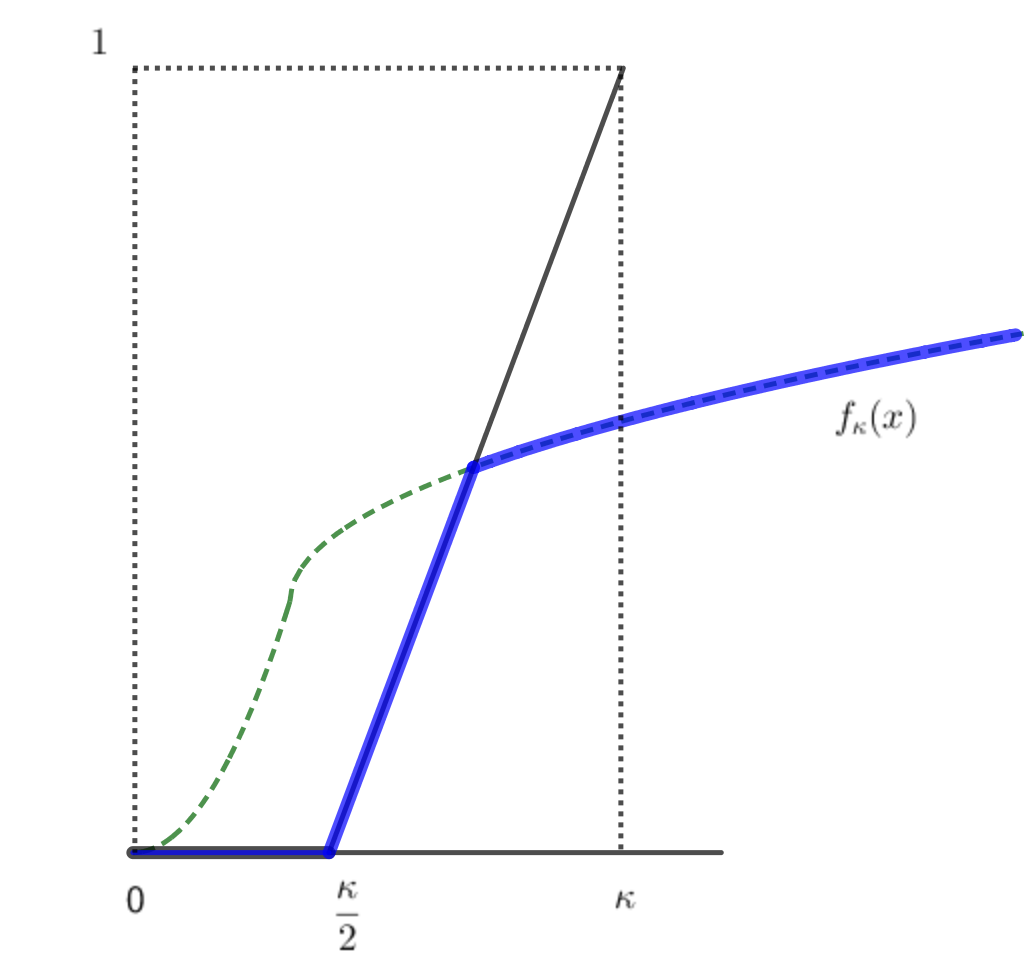
\includegraphics[scale=0.40]{Drafts and notes/fig1.png}
    \caption{Graph of the function $f_\kappa$.}
    \label{fig:f_kappa}
\end{figure}
A graph of $f_\kappa$ is given in Figure \ref{fig:f_kappa}. The continuity at $x\in \partial\Omega_\kappa$ comes from the fact that when $d(x) =\kappa$, we have $g_k(x) = L\kappa \geq f(x)$ by \eqref{e:bound_aa}. It is clear that $f_\kappa$ is Lipschitz with $\Vert f_\kappa\Vert_{L^\infty(\Omega)}\leq L$ as well and $f_\kappa\to f$ uniformly as $\kappa\to 0$. Indeed, we have $0\leq f_\kappa \leq f$ and
\begin{equation*}
    0\leq \max_{x\in \overline{\Omega}} (f(x) - f_\kappa(x)) \leq \max_{x\in \overline{\Omega}\backslash \overline{\Omega}_\kappa} (f(x) - f_\kappa(x)) = \max_{x\in \overline{\Omega}\backslash \overline{\Omega}_\kappa} f(x) \leq L\kappa.
\end{equation*}
Let $u^\varepsilon_\kappa\in \rmC^2(\Omega)\cap\rmC(\overline{\Omega})$ be the solution to \eqref{eq:PDEeps} with datum $f\chi_{\kappa}$ and $u_k\in \mathrm{C}(\overline{\Omega})$ be the corresponding solution to \eqref{eq:PDE0} with datum $f{\chi_\kappa}$. By comparison principle (\cite[Corollary II.1]{Lasry1989}) we have
\begin{equation}\label{e:bound_2aa}
    0\leq u^\varepsilon(x) - u^\varepsilon_\kappa(x) \leq L\kappa \qquad\text{for}\;x\in \Omega.
\end{equation}
By the comparison principle for \eqref{eq:PDE0}, we also have
\begin{equation}\label{e:bound_2ab}
    0\leq u(x) - u_\kappa(x) \leq L\kappa \qquad\text{for}\;x\in \Omega.
\end{equation}
If $1<p<2$, by Theorem \ref{thm:rate_doubling1}, there exists a constant $C$ independent of $\kappa$ such that
\begin{equation}\label{e:bound_2ac}
    -C\sqrt{\varepsilon}\leq u^\varepsilon_\kappa(x) - u_\kappa(x)\leq C\left[\sqrt{\varepsilon} + \left(\frac{\varepsilon}{\kappa}\right)^{\alpha+1} + \left(\frac{\varepsilon}{\kappa}\right)^{\alpha+2} + \frac{\varepsilon^{\alpha+1}}{d(x)^\alpha}\right], \qquad x\in \Omega.
\end{equation}
Combining \eqref{e:bound_2aa}, \eqref{e:bound_2ab} and \eqref{e:bound_2ac}, we obtain
\begin{equation*}
\begin{split}
   -C\sqrt{\varepsilon}\leq u^\varepsilon(x) - u(x) &= \Big(u^\varepsilon(x) - u^\varepsilon_\kappa(x)\Big) + \Big(u^\varepsilon_\kappa(x) - u_\kappa(x)\Big) + \Big(u_\kappa(x) - u(x)\Big) \\
    &\leq L\kappa + C\left[\sqrt{\varepsilon} + \left(\frac{\varepsilon}{\kappa}\right)^{\alpha+1} + \left(\frac{\varepsilon}{\kappa}\right)^{\alpha+2} + \frac{\varepsilon^{\alpha+1}}{d(x)^\alpha}\right], \qquad x\in \Omega.
\end{split}
\end{equation*}
Choose $\kappa = \sqrt{\varepsilon}$. We deduce that
\begin{equation*}
    -C\sqrt{\varepsilon}\leq u^\varepsilon(x) - u(x) \leq C\sqrt{\varepsilon} + \frac{C\varepsilon^{\alpha+1}}{d(x)^\alpha}
\end{equation*}
for $x\in \Omega$ and the conclusion follows. \\

\noindent If $p=2$, by Theorem \ref{thm:rate_doubling1}, there exists a constant $C$ independent of $\kappa$ such that
\begin{equation}\label{e:bound_2acp=2}
    -C\sqrt{\varepsilon}\leq u^\varepsilon_\kappa(x) - u_\kappa(x) \leq C\left[\sqrt{\varepsilon} + \varepsilon + \varepsilon |\log(\kappa)|+\left(\frac{\varepsilon}{\kappa}\right)^2 + \varepsilon\log\left(\frac{1}{d(x)}\right)\right], \qquad x\in \Omega.
\end{equation}
Combining \eqref{e:bound_2aa}, \eqref{e:bound_2ab} and \eqref{e:bound_2acp=2}, we obtain
\begin{equation*}
\begin{split}
   -C\sqrt{\varepsilon}\leq u^\varepsilon(x) - u(x) &= \Big(u^\varepsilon(x) - u^\varepsilon_\kappa(x)\Big) + \Big(u^\varepsilon_\kappa(x) - u_\kappa(x)\Big) + \Big(u_\kappa(x) - u(x)\Big) \\
    &\leq L\kappa + C\left[\sqrt{\varepsilon} + \varepsilon|\log(\kappa)| + \left(\frac{\varepsilon}{\kappa}\right)^{2} + \varepsilon\log\left(\frac{1}{d(x)}\right) \right], \qquad x\in \Omega.
\end{split}
\end{equation*}
Choose $\kappa = \varepsilon$. We deduce that
\begin{equation*}
    -C\sqrt{\varepsilon}\leq u^\varepsilon(x) - u(x) \leq C\sqrt{\varepsilon} +\varepsilon\log\left(\frac{1}{d(x)}\right)
\end{equation*}
for $x\in \Omega$ and the conclusion follows. 
\end{proof}


\subsection{An improved one-sided rate of convergence}
We still assume $f = 0$ on $\partial\Omega$ and $f\geq 0$ such that $f\in \rmC^2(\overline{\Omega})$. From Lemma \ref{lem:f=0} we have $u = 0$ on $\partial\Omega$. Extent $u$ to $\R^n$ by setting 
\begin{equation*}
    \tilde{u}(x) = \begin{cases}
      u(x) &\qquad\text{if}\;x\in \overline{\Omega},\\
      0 &\qquad\text{if}\;x\notin \overline{\Omega}.
    \end{cases}
\end{equation*}

\begin{lem} If $f = 0$ on $\partial\Omega$ then the extension $\tilde{u}$ is a viscosity solution to
\begin{equation*}
    \tilde{u}(x)+|D\tilde{u}(x)|^p - f(x) = 0 \qquad\text{in}\;\R^n.
\end{equation*}
As a consequence (Theorem \ref{convex}) $-D^2\tilde{u} \succ -c\;\mathbb{I}_n$ in $\R^n$ if $f\in \mathrm{C}_c^2(\R^n)$ and 
\begin{equation}\label{def_c}
    c = \max \big\lbrace  D_{\xi\xi}f(x): |\xi|=1, x\in \overline{\Omega} \big\rbrace\geq 0.
\end{equation}
\end{lem}
\begin{proof} We only need to check that the viscosity solution test hold for $\tilde{u}$ as $x\in \partial\Omega$. The supersolution test holds trivially since $f = \tilde{u} = 0$ on $\partial\Omega$. If $\varphi\in \mathrm{C}^1(\R^n)$ such that $\tilde{u} - \varphi$ has a local maximum at $x\in \partial\Omega$, then $\tilde{u}(y) - \tilde{u}(y) \leq - \tilde{u}(x)$ for all $y\in \R^n$. Since $u\geq 0$, we deduce that $\varphi$ has a local minimum at $x\in \partial\Omega$, therefore $\tilde{u}(x)+|D\varphi(x)|^p - f(x) = 0$ and thus the viscosity subsolution test is satisfied.
\end{proof}



\begin{thm}[Compactly supported data]\label{thm:rate_doubling2} Assume that $f\in \mathrm{C}^2_c(\Omega)$ such that $\mathrm{supp}(f)\subset\Omega_\kappa$ where $0<\kappa < \delta_{0}$. Let $u^\varepsilon$ be the unique solution to \eqref{eq:PDEeps} and $u$ be the unique solution to \eqref{eq:PDE0}. Then there exists a constant $C$ independent of $\varepsilon$ and $\kappa$ such that
\begin{equation*}
\begin{aligned}
    u^\varepsilon(x) - u(x) &\leq\frac{\nu C_\alpha \varepsilon^{\alpha+1}}{d(x)^\alpha} + CC_\frac{\kappa}{2} \left(\left(\frac{\varepsilon}{\kappa}\right)^{\alpha+1}+\left(\frac{\varepsilon}{\kappa}\right)^{\alpha+2}\right) + nc\varepsilon, \quad \text{if} \quad 1 < p <2, \\
    u^\varepsilon(x) - u(x) & \leq \nu \varepsilon \log\left( \frac{1}{d(x)}\right)+C C_\frac{\kappa}{2}\left(\frac{\varepsilon}{\kappa}\right) +C\left( \frac{\varepsilon}{\kappa}\right)^2 + nc \varepsilon, \quad \text{if} \quad p=2,
\end{aligned}
\end{equation*}
where $c$ is defined as in \eqref{def_c} and $C_\frac{\kappa}{2}$ is the gradient bound of $u^\varepsilon$ on $\overline{\Omega}_\frac{\kappa}{2}$ as in \eqref{e:priorie_eps}.
\end{thm}

\begin{proof} For $1<p<2$, we proceed as in the proof of Theorem \ref{thm:rate_doubling1} to obtain 
\begin{align}
    &0\leq u^\varepsilon(x) \leq \tilde{u}^\varepsilon(x)  \leq \frac{\nu C_\alpha\varepsilon^{\alpha+1}}{d_\kappa(x)^{\alpha}} + C_3\left(\frac{4\varepsilon}{\kappa}\right)^{\alpha+2} \label{annulus2a}
    %&0\leq u^\varepsilon(x)\leq \tilde{u}^\varepsilon(x) \leq \nu \varepsilon \log\left(\frac{1}{d_\kappa(x)}\right)+C_\nu\left(\frac{4\varepsilon}{\kappa}\right)^{2}\qquad\text{for}\;p=2,\label{annulus2p=2a}
\end{align}
for $x\in U_\kappa$. Let
\begin{equation*}
    \psi^\varepsilon(x) := u^\varepsilon(x) - \frac{\nu C_\alpha \varepsilon^{\alpha+1}}{d(x)^\alpha}, \qquad x\in \Omega
\end{equation*}
where $\nu > 1$ is chosen as in Lemma \ref{lem:super_refined}. It is clear that $u-\psi^\varepsilon$ has a local minimum at some point $x_0\in \Omega$ since $\psi^\varepsilon(x)\to -\infty$ as $x\to \partial\Omega$. The normal derivative test gives us 
\begin{equation*}
    D\psi^\varepsilon(x_0) = Du^\varepsilon(x_0) + \nu C_\alpha\alpha \left(\frac{\varepsilon}{d(x_0)}\right)^{\alpha+1} D d(x_0) \in D^-u(x_0).
\end{equation*}
There are two cases to consider:
\begin{itemize}
    \item If $\displaystyle d(x_0)< \frac{1}{2}\kappa$, then as in the proof of Theorem \ref{thm:rate_doubling1}, $x_0\in U_\kappa$ and $d_\kappa(x_0) = d(x_0)$. By the definition of $x_0$, for any $x\in \Omega$, there holds
    \begin{align*}
        u(x) - \left(u^\varepsilon(x) - \frac{\nu C_\alpha \varepsilon^{\alpha+1}}{d(x)^\alpha}\right) \geq u(x_0) - \left(u^\varepsilon(x_0) - \frac{\nu C_\alpha \varepsilon^{\alpha+1}}{d(x_0)^\alpha}\right).
    \end{align*}
    Therefore,
    \begin{equation*}
    \begin{split}
        u^\varepsilon(x) - u(x) - \frac{\nu C_\alpha \varepsilon^{\alpha+1}}{d(x)^\alpha} &\leq  \left(u^\varepsilon(x_0) - \frac{\nu C_\alpha \varepsilon^{\alpha+1}}{d(x_0)^\alpha}\right) - u(x_0) \leq C_3 \left(\frac{4\varepsilon}{\kappa}\right)^{\alpha+2}
    \end{split}
    \end{equation*}
    thanks to \eqref{annulus2a}. Thus, in this case
    \begin{equation*}
        u^\varepsilon(x) - u(x) \leq \frac{\nu C_\alpha \varepsilon^{\alpha+1}}{d(x)^\alpha} + C_3 \left(\frac{4\varepsilon}{\kappa}\right)^{\alpha+2}, \qquad x\in \Omega.
    \end{equation*}
    \item If $\displaystyle d(x_0) \geq \frac{1}{2}\kappa$, from the fact that $u$ is semiconcave in $\Omega$, 
\begin{equation*}
    D^2\psi^\varepsilon(x_0) \prec c\;\mathbb{I}_n
\end{equation*}
which implies that
\begin{equation*}
    \Delta \psi^\varepsilon(x_0) \leq nc.
\end{equation*}
In other words, we have
\begin{equation*}
    \varepsilon\Delta u^\varepsilon (x_0) - \frac{\nu C_\alpha \alpha(\alpha+1)\varepsilon^{\alpha+2}}{d(x_0)^{\alpha+2}}| Dd(x_0)|^2 + \frac{\nu C_\alpha \alpha \varepsilon^{\alpha+2}}{d(x_0)^{\alpha+1}}\Delta d(x_0) \leq nc\varepsilon.
\end{equation*}
Since $d(x_0)\geq \frac{1}{2}\kappa$, we can further deduce that
\begin{equation}\label{delta_psi}
    \varepsilon\Delta u^\varepsilon(x_0) \leq nc\varepsilon + \frac{C\varepsilon^{\alpha+2}}{d(x_0)^{\alpha+2}} \leq nc\varepsilon +  C\left(\frac{\varepsilon}{\kappa}\right)^{\alpha+2}
\end{equation}
where $C$ is independent of $\varepsilon$. Since $\psi^\varepsilon\in \rmC^2(\Omega)$, the viscosity supersolution test for $u$ gives us
\begin{equation}\label{convex1}
    u(x_0) + \left|Du^\varepsilon(x_0) + \frac{\nu C_\alpha \alpha \varepsilon^{\alpha+1}}{d(x_0)^{\alpha+1}}D d(x_0)\right|^p - f(x_0) \geq 0.
\end{equation}
On the other hand, $u^\varepsilon$ solves
\begin{equation}\label{convex2}
    u^\varepsilon(x_0) + |Du^\varepsilon(x_0)|^p - f(x_0) - \varepsilon \Delta u^\varepsilon(x_0) = 0.
\end{equation}
Combine \eqref{convex1} and \eqref{convex2} to obtain that
\begin{align}\label{convex3}
    u^\varepsilon(x_0) - u(x_0) &\leq \left|Du^\varepsilon(x_0) + \frac{\nu C_\alpha \alpha \varepsilon^{\alpha+1}}{d(x_0)^{\alpha+1}}D d(x_0)\right|^p - |Du^\varepsilon(x_0)|^p + \varepsilon\Delta u^\varepsilon(x_0).
\end{align}
Now we estimate the gradient terms on the right hand side of \eqref{convex3}, i.e., 
\begin{align}\label{convex4}
    &\left|Du^\varepsilon(x_0) + \frac{\nu C_\alpha \alpha \varepsilon^{\alpha+1}}{d(x_0)^{\alpha+1}}D d(x_0)\right|^p - |Du^\varepsilon(x_0)|^p\nonumber \\
    &\qquad \qquad \leq p\left(|Du^\varepsilon(x_0)| + \frac{\nu C_\alpha \alpha \varepsilon^{\alpha+1}}{d(x_0)^{\alpha+1}}\left|D d(x_0)\right|\right)^{p-1} \frac{\nu C_\alpha \alpha \varepsilon^{\alpha+1}}{d(x_0)^{\alpha+1}}|D d(x_0)|\nonumber\\
    &\qquad \qquad \leq p\left(C_\frac{\kappa}{2} + C\left(\frac{\varepsilon}{\kappa}\right)^{\alpha+1}\right)^{p-1} C\left(\frac{\varepsilon}{\kappa}\right)^{\alpha+1}\nonumber\\
    &\qquad\qquad\leq CC_\frac{\kappa}{2}\left(1+\left(\frac{\varepsilon}{\kappa}\right)^{\alpha+1}\right)^{p-1} \left(\frac{\varepsilon}{\kappa}\right)^{\alpha+1} \leq CC_\frac{\kappa}{2} \left(\frac{\varepsilon}{\kappa}\right)^{\alpha+1}\left(1+ \left(\frac{\varepsilon}{\kappa}\right)\right)
\end{align}
where $C_\frac{\kappa}{2}$ is the upper bound of $Du^\varepsilon$ in $\Omega_\frac{\kappa}{2}$, as is given in the a priori estimate (Theorem \ref{thm:grad_1}) and $C$ is a constant that depends only on $\nu$, $\alpha$, and bounds on $d,Dd$ and $\Delta d$. Using \eqref{delta_psi} and \eqref{convex4} in \eqref{convex3}, we get
\begin{equation*}
    u^\varepsilon(x_0) - u(x_0) \leq nc\varepsilon + CC_\frac{\kappa}{2} \left(\frac{\varepsilon}{\kappa}\right)^{\alpha+1}\left(1+ \left(\frac{\varepsilon}{\kappa}\right)\right) + C\left(\frac{\varepsilon}{\kappa}\right)^{\alpha+2}.
\end{equation*}
%\textcolor{orange}{(I feel you missed some terms when estimating $\epsilon \Delta u^\epsilon$, because $\Delta \psi \neq \Delta u^\epsilon$. But it won't affect the result.)}

Therefore, in this case 
\begin{equation*}
    u^\varepsilon(x) - u(x) \leq \frac{\nu C_\alpha \varepsilon^{\alpha+1}}{d(x)^\alpha} + CC_\frac{\kappa}{2} \left(\frac{\varepsilon}{\kappa}\right)^{\alpha+1}\left(1+ \left(\frac{\varepsilon}{\kappa}\right)\right) + nc\varepsilon, \qquad x\in \Omega.
\end{equation*}
\end{itemize}
From the two cases, the conclusion follows. 

For $p = 2$, the argument is similar. We take $\psi^\varepsilon(x):=u^\varepsilon(x)-\nu \varepsilon \log \left(\frac{1}{d(x)}\right)$ instead and still $u-\psi^\varepsilon$ attains a local minimum at some point $x_0 \in \Omega$. Carrying out the similar computations as in the case of $1 < p < 2$, we have:
\begin{itemize}
    \item If $\displaystyle d(x_0) < \frac{1}{2} \kappa$, then
    \begin{equation*}
        u^\varepsilon(x)-u(x) \leq \nu \varepsilon \log \left( \frac{1}{d(x)} \right) + C\left( \frac{4\varepsilon}{\kappa}\right)^2, \quad x \in \Omega.
    \end{equation*}
    \item If $\displaystyle d(x_0) \geq \frac{1}{2} \kappa$, then
    \begin{equation*}
        u^\varepsilon(x)-u(x) \leq \nu \varepsilon \log\left(\frac{1}{d(x)}\right) + 
        C C_\frac{\kappa}{2} \left( \frac{\varepsilon}{\kappa} \right) + C \left( \frac{\varepsilon}{\kappa} \right)^2 + nc\varepsilon, \quad x \in \Omega.
    \end{equation*}
\end{itemize}
Therefore, the conclusion follows.
\end{proof}

\begin{rem} Using our approach, in order to relax the assumption $\mathrm{supp}(f)\subset\subset\Omega$ to $f = 0$ on $\partial\Omega$ as in Theorem \ref{main_thm1}, we need to know more about the blow up rate $C_\kappa$ in $|Du^\varepsilon(x)|\leq C_\kappa$ as $\kappa\to 0$. We will use the result in 

\end{rem}

\begin{cor} Assume $f = 0$ on $\partial\Omega$. Let $u^\varepsilon$ be the unique solution to \eqref{eq:PDEeps} and $u$ be the unique solution to \eqref{eq:PDE0}. Let $K$ be a compact subset of $\Omega$, then there exists a constant $C_K$ such that 
\begin{equation*}
    \sup_{x\in K} \big(u^\varepsilon(x) -u(x)\big) \leq C_K\varepsilon.
\end{equation*}
\end{cor}
\begin{proof} We can find $\kappa\in \left(0,\delta_0\right)$ such that $K\subset\subset \Omega_{\kappa}$. Define $f_\kappa$ as in the proof of Theorem \ref{main_thm1}, where $\mathrm{supp}(f_\kappa)\subset\Omega_{\frac{\kappa}{2}}$ and
\begin{equation*}
    0\leq f - f_\kappa \leq L\kappa
\end{equation*}
where $L$ is the Lipschitz constant of $f$. Let $u^\varepsilon_\kappa\in \rmC^2(\Omega)\cap \rmC(\overline{\Omega})$ be the solution to \eqref{eq:PDEeps} with datum $f_k$ and $u_k$ be the solution to \eqref{eq:PDE0} with datum $f_k$, then
\begin{equation*}
  0\leq u^\varepsilon(x) - u^\varepsilon_\kappa(x)\leq L\kappa \qquad\text{for}\;x\in \Omega
\end{equation*}
and
\begin{equation*}
    0\leq u(x) - u_\kappa(x)\leq L\kappa \qquad\text{for}\;x\in \Omega.
\end{equation*}
Therefore
\begin{equation*}
    u^\varepsilon(x)-u(x)\leq 2L\kappa + \big(u^\varepsilon_\kappa - u_\kappa\big) \leq 2L\kappa+C_{\kappa}\varepsilon
\end{equation*}
where we use the rate $\mathcal{O}(\varepsilon)$ from Theorem \ref{thm:rate_doubling2} as $f_\kappa$ is compactly supported. 
\end{proof}


\begin{rem} It is clear from the proof that $C_K$ blows up as $K$ approaching $\Omega$ and we do not have any boundary layer yet, since the bound $|Du^\varepsilon(x)|\leq C_\kappa$ for $x\in \Omega_\kappa$ is not an explicit bound. We refer the readers to \cite{alessio_asymptotic_2006} for an explicit behavior of $Du^\varepsilon(x)$ as $x\to \partial \Omega$. Of course, using this explicit behavior of $Du^\varepsilon$ we can obtain a boundary layer from this proof, which we omit it here.
\end{rem}




\begin{proof}[Proof of Theorem \ref{main_thm2}] Define 

\end{proof}


%\clearpage


%\section{Rate of convergence via nonlinear adjoint method}

%\begin{appendices}
\section*{Appendix}
\subsection*{Estimates on solutions}
We present here a proof for the gradient bound of solution to \eqref{eq:PDEeps} using the Bernstein method (see also \cite{Lasry1989,lions_quelques_1985}). Another proof using a different technique is given in \cite{Armstrong2015a}.

\begin{proof}[Proof of Theorem \ref{thm:grad_1}] Let $\theta\in (0,1)$ be chosen later, $\varphi\in \mathrm{C}_c^\infty(\Omega)$, $0\leq \varphi\leq 1$, $\mathrm{supp}\;\varphi\subset \Omega$ and $\varphi = 1$ on $\Omega_\delta$ such that there exists $C = C(\delta,\theta)$,
\begin{equation}\label{e:ass_power}
    |\Delta \varphi(x)| \leq C\varphi^\theta \qquad\text{and}\qquad |D \varphi(x)|^2 \leq C\varphi^{1+\theta}
\end{equation}
for all $x\in \Omega$.
Define $w(x) := |Du(x)|^2$ for $x \in \Omega$. The equation for $w$ is given by
\begin{equation*}
    -\varepsilon \Delta w + 2 p|D u|^{p-2}D u \cdot D w + 2  w - 2 D f\cdot D u + 2 \varepsilon |D^2u|^2 = 0 \qquad\text{in}\;\Omega.
\end{equation*}
%\textcolor{orange}{(I think the coefficients here are not correct. I put the corrected ones in orange. Originally, all the coefficients were 1 except for the term 2w.)}

Then an equation for $(\varphi w)$ can be derived as follows.
\begin{align*}
    &-\varepsilon \Delta (\varphi w) + 2 p|D u|^{p-2}D u \cdot D (\varphi w) + 2  (\varphi w) + 2 \varepsilon \varphi|D^2u|^2 + 2\varepsilon \frac{D \varphi}{\varphi}\cdot D (\varphi w) \\
    &\qquad\qquad\qquad\qquad = \varphi(D f\cdot D u) + 2 p|D u|^{p-2}(D u\cdot D \varphi)w -\varepsilon w \Delta \varphi + 2\varepsilon \frac{|D \varphi|^2}{\varphi}w
    \qquad\text{in}\;\mathrm{supp}\;\varphi.
\end{align*}
Assume that $\varphi w$ achieves its maximum over $\overline{\Omega}$ at $x_0\in \Omega$. And we can further assume that $x_0\in \mathrm{supp}\;\varphi$, since otherwise the maximum of $\varphi w$ over $\overline{\Omega}$ is zero. By the classical maximum principle, 
\begin{equation*}
    -\varepsilon \Delta(\varphi w)(x_0)\geq 0 \qquad\text{and}\qquad |D(\varphi w)(x_0)| = 0.
\end{equation*}
Use this in the equation of $\varphi w$ above to obtain
\begin{equation*}
    \varepsilon \varphi|D^2u|^2 \leq  \varphi (Df\cdot Du)+ 2 p|Du|^{p-1} |D\varphi|w + \varepsilon w |\Delta\varphi|  + 2\varepsilon  w\frac{|D\varphi|^2}{\varphi},
\end{equation*}
 where all terms are evaluated at $x_0$. From \eqref{e:ass_power}, we have
\begin{equation}\label{e:est_for_D^2u}
    \varepsilon \varphi|D^2u|^2 \leq  \varphi |Df|w^{\frac{1}{2}}+ 2 Cp w^{\frac{p-1}{2}+1} \varphi^{\frac{1+\theta}{2}} + C\varepsilon w \varphi^{\theta} + 2C\varepsilon  w\varphi^\theta.
\end{equation}
By Cauchy-Schwartz inquality, $n|D^2u|^2\geq (\Delta u)^2$. Thus, if $n\varepsilon < 1$, then
\begin{equation}\label{e:est_for_D^2u_2}
    \varepsilon |D^2u|^2 \geq \frac{(\varepsilon \Delta u)^2}{n\varepsilon} \geq (\varepsilon \Delta u)^2 = \left(  u + |Du|^p - f\right)^2 \geq |Du|^{2p} - 2C|Du|^p \geq \frac{|Du|^{2p}}{2} - 2C
\end{equation}
where $C$ depends on $\max_{\overline{\Omega}}f$ only. Using \eqref{e:est_for_D^2u_2} in \eqref{e:est_for_D^2u}, we obtain that
\begin{equation*}
    \varphi\left(\frac{1}{2}w^p - 2C\right) \leq \varphi |Df|w^{\frac{1}{2}}+ 2 Cp w^{\frac{p-1}{2}+1} \varphi^{\frac{1+\theta}{2}} + 3C\varepsilon w \varphi^{\theta}.
\end{equation*}
Multiply both sides by $\varphi^{p-1}$ to deduce that
\begin{align*}
    (\varphi w)^p \leq 4C\varphi^{p-1} + 2\Vert Df\Vert_{L^\infty}\varphi^p w^{\frac{1}{2}} + 4Cp \varphi^{\frac{2p+\theta - 1}{2}}w^{\frac{p+1}{2}} + 6C\varepsilon \varphi^{p+\theta - 1}w.
\end{align*}
Choose $2p+\theta -1 \geq p+1$, i.e., $p+\theta\geq 2$. This is always possible with the requirement $\theta \in (0,1)$, as $1<p <\infty$. Then we get
\begin{equation}\label{e:est_for_D^2u_3}
    (\varphi w)^p \leq C\left(1+ (\varphi w)^\frac{1}{2} + (\varphi w)^\frac{p+1}{2} +(\varphi w)\right).
\end{equation}
As a polynomial in $z = (\varphi w)(x_0)$, this implies that $(\varphi w)(x_0)\leq C$ where $C$ depends on coefficients of the right hand side of \eqref{e:est_for_D^2u_3}, which gives our desired gradient bound since $\overline{\Omega}_\delta\subset \mathrm{supp}\;\varphi$.
\end{proof}

\subsection*{Asymptotic behavior of derivatives}
We denote by $\nu(x)$ the outward unit normal vector at any point $x\in \partial{\Omega}$ and $\tau(x)$ the unitary tangent vector defined on $\partial{\Omega}$, i.e., $\nu(x)\cdot\tau(x) = 0$. We start by considering the case $p=2$.
\begin{equation*}
    \begin{cases}
    -\Delta u 
    \end{cases}
\end{equation*}


\subsection*{Existence and wellposedness of solution}
\begin{proof} [Proof of Theorem \ref{thm:wellposed1<p<2}] If $p\in (1,2)$, we use the ansatz $ u(x) = C_\varepsilon d(x)^{-\alpha}$ to find a solution for \eqref{eq:PDEeps}. Plug the ansatz into \eqref{eq:PDEeps} and compute 
\begin{equation*}
    |Du (x)|^p = \frac{(\alpha C_\varepsilon)^p }{d(x)^{p(\alpha+1)}}|D d(x)|^p \qquad\text{and}\qquad\varepsilon\Delta u(x) = \frac{\varepsilon C_\varepsilon\alpha(\alpha+1)}{d(x)^{\alpha+2}}|D d(x)|^2 - \frac{\varepsilon C_\varepsilon\alpha}{d(x)^{\alpha+1}}\Delta d(x).
\end{equation*}
Since $|D d(x)| = 1$ for $x$ near $\partial\Omega$, as $x\to \partial \Omega$, the explosive terms of the highest order are
\begin{equation*}
         C_\varepsilon^p \alpha^p d^{-(\alpha+1)p}  -\varepsilon C_\varepsilon \alpha(\alpha+1)d^{-(\alpha+2)}.
\end{equation*}
Set the above to be zero to obtain that
\begin{equation}\label{e:relation}
    \displaystyle\alpha = \frac{2-p}{p-1} \qquad\text{and}\qquad C_\varepsilon = \left(\frac{1}{\alpha}(\alpha+1)^\frac{1}{p-1}\right) \varepsilon^{\frac{1}{p-1}} = \frac{1}{\alpha}(\alpha+1)^{\alpha+1}\varepsilon^{\alpha+1}.
\end{equation}
For $0<\delta < \frac{1}{2}\delta_0$ and $\eta$ small, define
\begin{equation*}
\begin{split}
    \overline{w}_{\eta,\delta}(x) &:= \frac{(C_\alpha+\eta)\varepsilon^{\alpha+1}}{(d(x)-\delta)^\alpha} + M_\eta, \qquad x\in \Omega_\delta,\\
    \underline{w}_{\eta,\delta}(x) &:= \frac{(C_\alpha-\eta)\varepsilon^{\alpha+1}}{(d(x)+\delta)^\alpha} - M_\eta, \qquad x\in \Omega^\delta,
\end{split}
\end{equation*}
where $C_\alpha := \frac{1}{\alpha} (\alpha+1)^{\alpha+1} $, $M_\eta$ to be chosen. We will show that $\overline{w}_{\eta,\delta}$ is a supersolution of \eqref{eq:PDEeps} in $\Omega_\delta$, while $\underline{w}_{\eta,\delta}$ is a subsolution of \eqref{eq:PDEeps} in $\Omega^\delta$. Compute
\begin{align*}
    \mathcal{L}^\varepsilon\left[\overline{w}_{\eta,\delta}\right](x) &= \frac{ (C_\alpha + \eta)\varepsilon^{\alpha+1}}{(d(x)-\delta)^\alpha} + M_\eta + \frac{(C_\alpha+\eta)^p \alpha^p\varepsilon^{\alpha+2}}{(d(x)-\delta)^{\alpha+2}}|D d(x)|^p - f(x) \\
    & \qquad\qquad\qquad\qquad\qquad - \frac{(C_\alpha+\eta)\alpha(\alpha+1)\varepsilon^{\alpha+2}}{(d(x)-\delta)^{\alpha+2}}|D d(x)|^2 + \frac{(C_\alpha+\eta)\alpha \varepsilon^{\alpha+2}}{(d(x)-\delta)^{\alpha+1}}\Delta d(x)\\
    &\geq M_\eta - f(x) + \underbrace{\frac{\nu C_\alpha\alpha(\alpha+1)\varepsilon^{\alpha+2}}{(d(x)-\delta)^{\alpha+2}}\left[\nu^{p-1}|Dd(x)|^{p} - |Dd(x)|^2 + \frac{(d(x)-\delta)\Delta d(x)}{\alpha+1}\right]}_{I}
\end{align*}
%\textcolor{orange}{(In the parenthesis of I, I think the first term should be $\nu^{p-1}|Dd(x)|^p$ instead of $\nu^{p-1}|Dd(x)|^{p-1}$.)}
where we use $(C_\alpha\alpha)^p = C_\alpha\alpha(\alpha+1)$ and $\nu = \frac{C_\alpha+\eta}{C_\alpha} \in (1,2)$ for small $\eta$. Let
\begin{equation*}
    \delta_\eta : = \frac{\alpha+1}{K_2}\left[\nu^{p-1}-1\right]
\end{equation*}
and $\delta_\eta \to 0$ as $\eta \to 0$.
Recall the definitions in \eqref{boundond}. To get  $\mathcal{L}^\varepsilon\left[\overline{w}_{\eta,\delta}\right]\geq 0$, there are two cases to consider, depending on how large $d(x)-\delta$ is.
\begin{itemize}
    \item If $0< d(x)-\delta <\delta_\eta < \delta_0$ for $\eta$ small and fixed, then $|Dd(x)| = 1$, and thus $I\geq 0$. Hence $\mathcal{L}^\varepsilon\left[\overline{w}_{\eta,\delta}\right]\geq 0$ if we choose $M_\eta \geq \max_{\overline{\Omega}} f$.
    %\textcolor{orange}{(Question: Here, $\eta$ is fixed right?)}
    \item If $d(x)-\delta\geq \delta_\eta$, then 
    \begin{equation*}
        I \leq \left(\frac{1}{\delta_\eta}\right)^{\alpha+2}\nu C_\alpha \alpha(\alpha+1)\left[\nu^{p-1}K_1^{p}+K_1^2+K_2K_0\right]\varepsilon^{\alpha+2}.
    \end{equation*}
    %\textcolor{orange}{(The first term in the bracket should be $\nu^{p-1}K_1^p$ instead of $\nu^{p-1}K_1^{p-1}$.)}
    
    Thus, we can choose $M_\eta = \max_{\overline{\Omega}} f + C\varepsilon^{\alpha+2}$ for $C$ large enough (depending on $\eta$) so that  $\mathcal{L}^\varepsilon\left[\overline{w}_{\eta,\delta}\right]\geq 0$.
\end{itemize}
Therefore, $\overline{w}_{\eta,\delta}$ is a supersolution in $\Omega_\delta$. 

Similarly, we have 
\begin{align*}
    \mathcal{L}_\varepsilon\left[\underline{w}_{\eta,\delta}\right](x) &= \frac{ (C_\alpha - \eta)\varepsilon^{\alpha+1}}{(d(x)+\delta)^\alpha} - M_\eta + \frac{(C_\alpha-\eta)^p \alpha^p\varepsilon^{\alpha+2}}{(d(x)+\delta)^{\alpha+2}}|D d(x)|^p - f(x) \\
    & \qquad\qquad\qquad\qquad\qquad - \frac{(C_\alpha-\eta)\alpha(\alpha+1)\varepsilon^{\alpha+2}}{(d(x)+\delta)^{\alpha+2}}|D d(x)|^2 + \frac{(C_\alpha-\eta)\alpha \varepsilon^{\alpha+2}}{(d(x)+\delta)^{\alpha+1}}\Delta d(x)\\
    &= - M_\eta - f(x) \\
    &+\underbrace{\frac{\nu C_\alpha\alpha(\alpha+1)\varepsilon^{\alpha+2}}{(d(x)+\delta)^{\alpha+2}}\left[\nu^{p-1}|Dd(x)|^{p} - |Dd(x)|^2 + \frac{(d(x)+\delta)\Delta d(x)}{\alpha+1}+\frac{(d(x)+\delta)^2}{\alpha(\alpha+1)\varepsilon}\right]}_{J}
\end{align*}
%\textcolor{orange}{(In the parenthesis of J, the first term should be $\nu^{p-1}|Dd(x)|^p$ instead of $\nu^{p-1}|Dd(x)|^{p-1}$.)}

where $\nu = \frac{C_\alpha-\eta}{C_\alpha}\in (0,1)$ for small $\eta$. Let
\begin{equation*}
    \delta_\eta := \left(1-\nu^{p-1}\right)\left(\frac{\alpha(\alpha+1)\varepsilon}{1+K_2\alpha\varepsilon}\right) 
\end{equation*}
%\textcolor{orange}{( $\delta_\eta := \left(1-\nu^{p-1}\right)\left(\frac{\alpha(\alpha+1)\varepsilon}{1+K_2\alpha\varepsilon}\right)$)}

and $\delta_\eta \to 0$ as $ \eta \to 0$.
To obtain $\mathcal{L}^\varepsilon\left[\underline{w}_{\eta,\delta}\right]\leq 0$, there are two cases to consider depending on how large $d(x)+\delta$ is.
\begin{itemize}
    \item If $0<d(x)+\delta<\delta_\eta < \delta_0$ for $\eta$ small and fixed, then $|Dd(x)| = 1$ , and thus $J\leq 0$. Hence $\mathcal{L}^\varepsilon\left[\underline{w}_{\eta,\delta}\right]\leq 0$ if we choose $M_\eta \geq -\max_{\Omega}f$.
    \item If $d(x)+\delta\geq \delta_\eta$, then
    \begin{equation*}
        |J|\leq \left(\frac{1}{\delta_\eta}\right)^{\alpha+2} \nu C_\alpha\alpha(\alpha+1)\left[\nu^{p-1}K_1^{p}+K_1^2 + \frac{(K_0+1)K_2}{\alpha+1} + \frac{(K_0+1)^2}{\alpha(\alpha+1)\varepsilon}\right]\varepsilon^{\alpha+2}
    \end{equation*}
    %\textcolor{orange}{($|J|\leq \left(\frac{1}{\delta_\eta}\right)^{\alpha+2} \nu C_\alpha\alpha(\alpha+1)\left[K_1^{p}+K_1^2 + \frac{(K_0+\delta)K_2}{\alpha+1} + \frac{(K_0+\delta)^2}{\alpha(\alpha+1)\varepsilon}\right]\varepsilon^{\alpha+2}$)}
    
     Thus, we can choose $M_\eta = -\max_{\overline{\Omega}} f - C\varepsilon^{\alpha+2}$ for $C$ large enough (depending on $\eta$) so that $\mathcal{L}^\varepsilon\left[\underline{w}_{\eta,\delta}\right]\leq 0$.
\end{itemize}
Therefore, $\underline{w}_{\eta,\delta}$ is a subsolution in $\Omega^\delta$.

For $p=2$, we use the ansatz $u(x) = -C_\varepsilon \log(d(x))$ instead. Similar to the previous case, one can find $u(x) = -\varepsilon\log(d(x))$. For $0<\delta<\frac{1}{2}\delta_0$,  define 
\begin{equation*}
    \begin{split}
        &\overline{w}_{\eta,\delta}(x) = -(1+\eta)\varepsilon\log(d(x)-\delta) + M_\eta, \qquad x\in \Omega_\delta,\\
        &\underline{w}_{\eta,\delta}(x) = -(1-\eta)\varepsilon\log(d(x)+\delta) - M_\eta, \qquad x\in \Omega^\delta,
    \end{split}
\end{equation*}
where $M_\eta$ is to be chosen so that $\overline{w}_{\eta,\delta}(x)$ is a supersolution in $\Omega_\delta$ and $\underline{w}_{\eta,\delta}$ is a subsolution in $\Omega^\delta$. The computations are omitted here, as they are similar to the previous case.
\smallskip

\noindent We divide the rest of the proof into 3 steps. We first construct a minimal solution, then a maximal solution to \eqref{eq:PDEeps}, and finally show that they are equal to conclude the existence and the uniqueness of the solution to \eqref{eq:PDEeps}.
\smallskip

\paragraph{\textbf{Step 1.}} There exists a minimal solution $\underline{u}\in \mathrm{C}^2(\Omega)$ of \eqref{eq:PDEeps} such that $v\geq \underline{u}$ for any other solution $v\in \mathrm{C}^2(\Omega)$ solving \eqref{eq:PDEeps}.

\begin{proof} Let $w_{\eta,\delta}\in \mathrm{C}^2(\Omega)$ solve
    \begin{equation}\label{e:w_def}
    \begin{cases}
        \mathcal{L}^\varepsilon\left[w_{\eta,\delta}\right] = 0 &\qquad\text{in}\;\Omega,\\
        \qquad w_{\eta,\delta} = \underline{w}_{\eta,\delta} &\qquad\text{on}\;\partial\Omega.
    \end{cases}
    \end{equation}
    \begin{itemize}
        \item Fix $\eta>0$. As $\delta\to 0$, the value of $\underline{w}_{\eta,\delta}$ blows up on the boundary. Therefore, by the standard comparison principle for the second-order elliptic equation with Dirichlet boundary, $\delta_1 \leq  \delta_2$ implies $w_{\eta,\delta_1}\geq  w_{\eta,\delta_2}$ on $\overline{\Omega}$. 
        \item For $\delta'>0$, since $\underline{w}_{\eta,\delta'}$ is a subsolution in $\overline{\Omega}$ with finite boundary, 
            \begin{equation}\label{e:cp_delta1}
                0<\delta \leq \delta'\qquad\Longrightarrow\qquad \underline{w}_{\eta,\delta'} \leq w_{\eta_,\delta'}\leq w_{\eta,\delta} \qquad\text{on}\;\overline{\Omega}.
            \end{equation}
        \item Similarly, since $\overline{w}_{\eta,\delta'}$ is a supersolution on $\Omega_{\delta'}$ with infinity value on the boundary $\partial\Omega_{\delta'}$, by comparison principle,
            \begin{equation}\label{e:cp_delta2}
                w_{\eta,\delta} \leq \overline{w}_{\eta, \delta'} \qquad\text{in}\;\Omega_{\delta'} \qquad\Longrightarrow\qquad w_{\eta,\delta} \leq \overline{w}_{\eta,0} \qquad\text{in}\;\Omega.
            \end{equation}
    \end{itemize}
    \noindent From \eqref{e:cp_delta1} and \eqref{e:cp_delta2}, we have
    \begin{equation}\label{e:cp_delta3}
        0<\delta \leq \delta'\qquad\Longrightarrow\qquad \underline{w}_{\eta,\delta'} \leq w_{\eta_,\delta'}\leq w_{\eta,\delta} \leq \overline{w}_{\eta,0} \qquad\text{in}\;\Omega.
    \end{equation}
    Thus, $\{w_{\eta,\delta}\}_{\delta>0}$ is locally bounded in $L^{\infty}_{\mathrm{loc}}(\Omega)$ ($\{w_{\eta,\delta}\}_{\delta>0}$ is uniformly bounded from below). Using the local gradient estimate for $w_{\eta,\delta}$ solving \eqref{e:w_def}, we deduce that $\{w_{\eta,\delta}\}_{\delta>0}$ is locally bounded in $W^{1,\infty}_{\mathrm{loc}}(\Omega)$. Since $w_{\eta,\delta}$ solves \eqref{e:w_def}, we further have that $\{w_{\eta,\delta}\}_{\delta>0}$ is locally bounded in $W^{2,r}_{\mathrm{loc}}(\Omega)$ for all $r<\infty$ by Calderon-Zygmund estimates.
    
    \noindent Local boundedness of $\{w_{\eta,\delta}\}_{\delta>0}$ in $W^{2,r}_{\mathrm{loc}}(\Omega)$ implies weak$^*$ compactness, that is, there exists a function $u\in W^{2,r}_{\mathrm{loc}}(\Omega)$ such that (via subsequence and monotonicity)
    \begin{equation*}
        w_{\eta,\delta} \rup u \qquad\text{weakly in}\;W^{2,r}_{\mathrm{loc}}(\Omega),\qquad \text{and}\qquad
        w_{\eta,\delta} \to u \qquad\text{strongly in}\;W^{1,r}_{\mathrm{loc}}(\Omega).
    \end{equation*}
    In particular, $w_{\eta,\delta}\to u$ in $\mathrm{C}^1_{\mathrm{loc}}(\Omega)$ thanks to Sobolev compact embedding. Let us rewrite the equation $\mathcal{L}^\varepsilon\left[w_{\eta,\delta}\right] = 0$ as $\varepsilon\Delta w_{\eta,\delta}(x) = F[w_{\eta,\delta}](x)$ for $x \in U\subset\subset \Omega$, where
    \begin{equation*}
        F[w_{\eta,\delta}](x) =    w_{\eta,\delta}(x) + H(x,Dw_{\eta,\delta}(x)).
    \end{equation*}
    Since $w_{\eta,\delta}\to u$ in $\mathrm{C}^1(U)$ as $\delta \to 0$, we have $F[w_{\eta,\delta}](x) \to F(x)$ uniformly in $U$ as $\delta \to 0$,  where 
    \begin{equation*}
        F(x) =   u(x) + H(x,Du(x)).
    \end{equation*}
    In the limit, we obtain that $u\in L^2(U)$ is a weak solution of $\varepsilon\Delta u = F$ in $U$ where $F$ is continuous. Thus, $u\in \mathrm{C}^2(\Omega)$ and by stability, $u$ solves $\mathcal{L}^\varepsilon[u] = 0$ in $\Omega$. From \eqref{e:cp_delta3}, we also have
    \begin{equation*}
        \underline{w}_{\eta,0} \leq u \leq \overline{w}_{\eta,0} \qquad\text{in}\;\Omega.
    \end{equation*}
    Moreover, $u(x)\to \infty$ as $\mathrm{dist}(x,\partial\Omega)\to 0$ with the precise rate like \eqref{rate_p<2} or \eqref{rate_p=2}. Note that by construction, $u$ may depend on $\eta$. But next, we will show that $u$ is independent of $\eta$, by proving $u$ is the unique minimal solution of $\mathcal{L}^\varepsilon[u] = 0$ in $\Omega$ with $u = +\infty$ on $\partial\Omega$.
    
    \noindent Let $v\in \rmC^{2}(\Omega)$ be a solution to \eqref{eq:PDEeps}. Fix $\delta>0$. Since $v(x)\to \infty$ as $x\to \partial\Omega$ while $w_{\eta,\delta}$ remains bounded on $\partial \Omega$, the comparison principle yields
    \begin{equation*}
        v\geq w_{\eta,\delta} \qquad\text{in} \; \Omega.
    \end{equation*}
    Let $\delta\to 0$ and we deduce that $v\geq u$ in $\Omega$. This concludes that $u$ is the minimal solution in $\mathrm{C}^2(\Omega)(\forall\,r<\infty)$ and thus $u$ is independent of $\eta$. 
\end{proof}


\paragraph{\textbf{Step 2.}} There exists a maximal solution $\overline{u}\in \mathrm{C}^2(\Omega)$ of \eqref{eq:PDEeps} such that $v\leq \overline{u}$ for any other solution $v\in \mathrm{C}^2(\Omega)$ solving \eqref{eq:PDEeps}.


\begin{proof} For each $\delta>0$, let $u_\delta\in \mathrm{C}^2(\Omega_\delta)$ be the minimal solution to $\mathcal{L}^\varepsilon[u_\delta] = 0$ in $\Omega_\delta$ with $u_\delta = +\infty$ on $\partial\Omega_\delta$. By the comparison principle, for every $\eta>0$, there holds
\begin{equation*}
    \underline{w}_{\eta,\delta} \leq u_\delta \leq \overline{w}_{\eta,\delta} \qquad\text{in}\;\Omega_\delta,
\end{equation*}
and
\begin{equation*}
    0<\delta<\delta' \qquad \Longrightarrow\qquad u_\delta \leq u_\delta' \qquad\text{in}\;\Omega_{\delta'}.
\end{equation*}
The monotoniciy, together with the local boundedness of $\{u_\delta\}_{\delta>0}$ in $W^{2,r}_{\mathrm{loc}}(\Omega)$, implies that there exists $u\in W^{2,r}_{\mathrm{loc}}(\Omega)$ for all $r<\infty$ such that $u_\delta\to u$ strongly in $\rmC^1_{\mathrm{loc}}(\Omega)$. Using the equation $\mathcal{L}^\varepsilon [u_\delta] = 0$ in $\Omega_\delta$ and the regularity of Laplace's equation, we can further deduce that $u\in \mathrm{C}^2(\Omega)$ solves \eqref{eq:PDEeps} and 
\begin{equation*}
    \underline{w}_{\eta,0} \leq u\leq \overline{w}_{\eta,0} \qquad\text{in}\;\Omega
\end{equation*}
for all $\eta>0$. As $u_\delta$ is independent of $\eta$ by the previous argument in Step 1, it is clear that $u$ is also independent of $\eta$. Now we show that $u$ is the maximal solution of \eqref{eq:PDEeps}. Let $v\in\rmC^2(\Omega)$ solve \eqref{eq:PDEeps}. Clearly $v\leq u_\delta$ on $\Omega_\delta$. Therefore, as $\delta \to 0$, we have $v\leq u$.
\end{proof}
\noindent In conclusion, we have found a minimal solution $\underline{u}$ and a maximal solution $\overline{u}$ in $\rmC^2(\Omega)$ such that
\begin{equation}\label{e:chain}
    \underline{w}_{\eta,0} \leq \underline{u}\leq \overline{u}\leq \overline{w}_{\eta,0} \qquad\text{in}\;\Omega
\end{equation}
for any $\eta>0$. This extra parameter $\eta$ now enables us to show that $\overline{u} = \underline{u}$ in $\Omega$. The key ingredient here is the convexity in the gradient slot of the operator.
\smallskip
\paragraph{\textbf{Step 3.}} We have $\overline{u}\equiv \underline{u}$ in $\Omega$. Therefore, the solution to \eqref{eq:PDEeps} in $\mathrm{C}^2(\Omega)$ is unique.

\begin{proof} Let $\theta\in (0,1)$. Define $w_\theta = \theta \overline{u} + (1-\theta) \inf_{\Omega} f$. It can be verified that $w_\theta$ is a subsolution to \eqref{eq:PDEeps}. Then one may argue that by the comparison principle,
\begin{equation*}
    w_\theta = \theta \overline{u} + (1-\theta)\inf_{\Omega} f\leq \underline{u} \qquad\text{in}\;\Omega,
\end{equation*}
and conclude that $\overline{u} \leq \underline{u}$ by letting $\theta\to 1$. But we have to be careful here. As they are both explosive solutions, to use the comparison principle, we need to show that $w_\theta \leq \underline{u}$ in a neighborhood of $\partial\Omega$. From \eqref{e:chain}, we see that
\begin{align*}
    &1\leq \frac{\overline{u}(x)}{\underline{u}(x)} \leq \frac{\overline{w}_{\eta,0}(x)}{\underline{w}_{\eta,0}(x)} = \frac{(C_\alpha+\eta)+ M_\eta d(x)^\alpha}{(C_\alpha-\eta)- M_\eta d(x)^\alpha},& 1<p<2,\\
    &1 \leq \frac{\overline{u}(x)}{\underline{u}(x)} \leq \frac{\overline{w}_{\eta,0}(x)}{\underline{w}_{\eta,0}(x)} = \frac{-(1+\eta)\log(d(x)) + M_\eta}{-(1-\eta)\log(d(x))-M_\eta}, & p=2,
\end{align*}
for $x\in \Omega$. Hence
\begin{align*}
     &1\leq  \lim_{d(x)\to 0} \left(\frac{\overline{u}(x)}{\underline{u}(x)}\right) \leq \frac{C_\alpha+\eta}{C_\alpha-\eta}, & 1< p < 2,\\
     &1\leq  \lim_{d(x)\to 0} \left(\frac{\overline{u}(x)}{\underline{u}(x)}\right) \leq \frac{-(1+\eta)}{-(1-\eta)}, & p = 2.
\end{align*}
Since $\eta>0$ is chosen arbitrary, we obtain
\begin{equation*}
     \lim_{d(x)\to 0} \left(\frac{\overline{u}(x)}{\underline{u}(x)}\right) = 1.
\end{equation*}
 This means for any $\varsigma\in(0,1)$, there exists $\delta(\varsigma)>0$ small such that 
\begin{equation*}
\frac{\overline{u}(x)}{\underline{u}(x)}\leq (1+\varsigma)     \qquad \text{, i.e.,}\qquad \left(\frac{1}{1+\varsigma}\right)\overline{u}(x) \leq \underline{u}(x) \qquad\text{in}\; \Omega\backslash \Omega_\delta.
\end{equation*}
For a given $\theta\in (0,1)$, one can always choose $\varsigma$ small enough such that $(1+\varsigma)^{-1} > \theta$. Now we just choose $\theta$ close to $1$ so that $\underline{u}(x) \geq \theta \overline{u}(x) + (1-\theta)\left(\inf_\Omega f\right)$ for $x \in \Omega \setminus \Omega_\delta$ for some $\delta$ depending on $\theta$.
\end{proof}


\noindent This finishes the proof of the well-posedness of \eqref{eq:PDEeps} for $1<p\leq2$. 
\end{proof}


\begin{proof}[Proof of Lemma \ref{lem:max}] The proof is a variation of Perron's method (see \cite{Capuzzo-Dolcetta1990}) and we proceed by contradiction. Let $\varphi\in \rmC(\overline{\Omega})$ and $x_0\in \overline{\Omega}$ such that $u(x_0) = \varphi(x_0)$ and $u-\varphi$ has a global strict minimum over $\overline{\Omega}$ at $x_0$ with 
\begin{equation}\label{eq:max_a1}
      \varphi(x_0) + H(x_0,D\varphi(x_0)) < 0.
\end{equation}
Let $\varphi^\varepsilon(x) = \varphi(x) - |x-x_0|^2 + \varepsilon$ for $x\in \overline{\Omega}$. Let $\delta > 0$. We see that for $x\in \partial B(x_0,\delta)\cap \overline{\Omega}$,
\begin{equation*}
    \varphi^\varepsilon(x) = \varphi(x) - \delta^2 +\varepsilon \leq \varphi(x) - \varepsilon
\end{equation*}
if $2\varepsilon \leq \delta^2$. We observe that
\begin{equation*}
    \begin{split}
    \varphi^\varepsilon(x) - \varphi(x_0)  &= \varphi(x)-\varphi(x_0) + \varepsilon - |x-x_0|^2 \\
    D\varphi^\varepsilon(x) - D\varphi(x_0) &= D\varphi(x) - D\varphi(x_0) - 2(x-x_0)
    \end{split}
\end{equation*}
for $x\in B(x,\delta)\cap \overline{\Omega}$. By the continuity of $H(x,p)$ near $(x_0,D\varphi(x_0))$ and the fact that $\varphi\in \rmC^1(\overline{\Omega})$, we can deduce from \eqref{eq:max_a1} that if $\delta$ is small enough and $0<2\varepsilon < \delta^2$, then
\begin{equation}\label{eq:max_a2}
      \varphi^\varepsilon(x)+H(x,D\varphi^\varepsilon(x)) < 0 \qquad\text{for}\;x\in B(x_0,\delta)\cap \overline{\Omega}.
\end{equation}
We have found $\varphi^\varepsilon\in \mathrm{C}^1(\overline{\Omega})$ such that $\varphi^\varepsilon(x_0)>u(x_0)$, $\varphi^\varepsilon<u$ on $\partial B(x_0,\delta)\cap \overline{\Omega}$ and \eqref{eq:max_a2}. Let
\begin{equation*}
    \tilde{u}(x) = \begin{cases}
    \max \big\lbrace u(x),\varphi^\varepsilon(x) \big\rbrace &x\in B(x_0,\delta)\cap \overline{\Omega},\\
    u(x)&x\notin B(x_0,\delta)\cap \overline{\Omega}.\\
    \end{cases}
\end{equation*}
We see that $\tilde{u}\in \rmC(\overline{\Omega})$ is a subsolution of \eqref{eq:PDE0} in $\Omega$ with $\tilde{u}(x_0) > u(x_0)$, which is a contradiction. Thus, $u$ is a supersolution of \eqref{eq:PDE0} on $\overline{\Omega}$.
\end{proof}


\begin{thm}\label{convex} Let $H(x,p) = G(p)-f(x)$ where $G\geq 0$ with $G(0) = 0$ is a convex function from $\R^n\to\R^n$ and $f\in \mathrm{C}^2_c(\R^n)$. Let $u\in \mathrm{C}_c(\R^n)$ be a viscosity solution to $u+H(x,Du) = 0$ in $\R^n$. Then $u$ is semiconcave, i.e, $u$ is a viscosity solution of  $-D^2u \succ -c\;\mathbb{I}_n$ in $\R^n$ where 
\begin{equation*}
    c = \max \big\lbrace  D_{\xi\xi}f(x): |\xi|=1, x\in \overline{\Omega} \big\rbrace\geq 0.
\end{equation*}
\end{thm}
\begin{proof} Let us consider the auxiliary functional
\begin{equation*}
    \Phi(x,y,z) = u(x)-2u(y)+u(z) - \frac{\alpha}{2}|x-2y+z|^2 - \frac{c}{2}|y-x|^2-\frac{c}{2}|y-z|^2
\end{equation*}
for $(x,y,z)\in \R^n\times\R^n\times\R^n$. By a priori estimate, $u$ is bounded and Lipschitz, thus we can assume $\Phi$ achieves its maximum over $\R^n\times\R^n\times \R^n$ at $(x_\alpha,y_\alpha,z_\alpha)$. The viscosity solutions tests give us
\begin{align*}
    &u(x_\alpha) + G\big(p_\alpha+c(x_\alpha-y_\alpha)\big) \leq f(x_\alpha)\\
    &u(z_\alpha) + G\big(p_\alpha+c(z_\alpha-y_\alpha)\big) \leq f(z_\alpha)\\
    &u(y_\alpha) + G\left(p_\alpha+\frac{c}{2}(x_\alpha-y_\alpha) + \frac{c}{2}(z_\alpha-y_\alpha)\right) \geq f(y_\alpha),
\end{align*}
where $p_\alpha = \alpha(x_\alpha-2y_\alpha+z_\alpha)$. Using the convexity of $G$ we have
\begin{equation*}
    2G\left(p_\alpha+\frac{c}{2}(x_\alpha-y_\alpha) + \frac{c}{2}(z_\alpha-y_\alpha)\right) \leq G\big(p_\alpha+c(x_\alpha-y_\alpha)\big)  + G\big(p_\alpha+c(z_\alpha-y_\alpha)\big)
\end{equation*}
therefore
\begin{equation*}
    u(x_\alpha) - 2u(y_\alpha) + u(z_\alpha) \leq f(x_\alpha) - 2f(y_\alpha) + f(z_\alpha).
\end{equation*}
\begin{itemize}
    \item $\Phi(x_\alpha,y_\alpha,z_\alpha)\geq \Phi(0,0,0)$ gives us
    \begin{equation*}
        \frac{\alpha}{2}|x-2y+z|^2 + \frac{c}{2}|y-x|^2+\frac{c}{2}|y-z|^2 \leq C.
    \end{equation*}
    Thus we can assume $(x_\alpha-y_\alpha)\to h_0$ and $(y_\alpha-z_\alpha)\to h_0$ as $\alpha\to \infty$.
    \item $\Phi(x_\alpha,y_\alpha,z_\alpha )\geq \Phi(y_\alpha+h_0,y_\alpha,y_\alpha-h_0)$ gives us
    \begin{align*}
        u(x_\alpha)-2u(y_\alpha) + u(z_\alpha) - \frac{\alpha}{2}|x_\alpha - 2y_\alpha+z_\alpha|^2 - \frac{c}{2}|x_\alpha-y_\alpha|^2 - \frac{c}{2}|y_\alpha-z_\alpha|^2 \\
        \geq u(y_\alpha+h_0) - 2u(y_\alpha) + u(y_\alpha-h_0) - c|h_0|^2.
    \end{align*}
    Therefore, using the fact that $u$ is Lipschitz, we have
    \begin{equation*}
    \begin{split}
        \frac{\alpha}{2}|x_\alpha - 2y_\alpha+z_\alpha|^2 
        &\leq c\left(\frac{2|h_0|^2 - |x_\alpha-y_\alpha|^2 - |y_\alpha-z_\alpha|^2}{2}\right) \\
        &+ C\Big(|(x_\alpha-y_\alpha) - h_0| + |(z_\alpha - y_\alpha) + h_0|\Big) \to 0
    \end{split}
    \end{equation*}
    as $\alpha\to \infty$.
\end{itemize}
For any $x\in \R^n$, we have $\Phi(x_\alpha,y_\alpha,z_\alpha) \geq \Phi(x+h,x,x-h)$, thus
\begin{align*}
    u(x+h)-2u(x)+u(x-h)-c|h|^2 &\leq f(x_\alpha)-2f(y_\alpha) + f(z_\alpha) \\
    &- \frac{\alpha}{2}|x_\alpha - 2y_\alpha+z_\alpha|^2-\frac{c}{2}|y_\alpha-x_\alpha|^2-\frac{c}{2}|y_\alpha-z_\alpha|^2.
\end{align*}
If $\{y_\alpha\}$ is unbounded as $\alpha\to \infty$ then since $f\in \mathrm{C}_c^2(\R^n)$, we have $f(y_\alpha)\to 0$ as $\alpha\to \infty$. As a consequence, $x_\alpha,z_\alpha \to \infty$ as well and thus $f(x_\alpha)-2f(y_\alpha) + f(z_\alpha)\to 0$ as $\alpha\to \infty$. Therefore
\begin{equation*}
    u(x+h)-2u(x)+u(x-h)-c|h|^2 \leq 0.
\end{equation*}
If $\{y_\alpha\}$ is bounded, then $y_\alpha\to y_0$ as $\alpha\to \infty$, thus
\begin{equation*}
     u(x+h)-2u(x)+u(x-h)-c|h|^2 \leq f(y_0+h_0) - 2f(y_0) + f(y_0-h_0) -c|h_0|^2.
\end{equation*}
Let $\xi = h_0$, we have
\begin{equation*}
    \begin{cases}
      f(y_0+h_0) - f(y_0) = \int_0^1 D_\xi f(y_0 + t\xi)\cdot \xi dt\\
      f(y_0) - f(y_0-h_0)  = \int_0^1 D_\xi f(y_0 - t\xi)\cdot \xi dt.
    \end{cases}
\end{equation*}
Therefore
\begin{equation*}
\begin{split}
     f(y_0+h_0) - 2f(y_0) + f(y_0-h_0) &= \int_0^1 \Big(D_\xi f(y_0 + t\xi) - D_\xi f(y_0 - t\xi) \Big)\cdot \xi dt\\
     &= \int_0^1 \int_0^1 D^2_{\xi\xi} \xi \cdot f(y_0+st \xi)\cdot \xi\;dtds.
\end{split}
\end{equation*}
Therefore
\begin{equation*}
    |f(y_0+h_0) - 2f(y_0) + f(y_0-h_0)| \leq \left(\max_{|\xi|=1}D_{\xi\xi} f\right)|\xi|^2.
\end{equation*}
Hence
\begin{equation*}
    u(x+h)-2u(x)+u(x-h)-c|h|^2 \leq 0
\end{equation*}
and thus $u$ is semiconcave. It is easy to see that if $\varphi$ is smooth and $u-\varphi$ has a local min at $x$ then $D^2\varphi(x)\prec c\;\mathbb{I}$, thus $-D^2\varphi(x)\geq -c\;\mathbb{I}$.
\end{proof}
%\textcolor{orange}{(I double checked the proof of Jeff and I think his proof is fine. Actually we can choose $y_\alpha$ so that $\{y_\alpha\}$ is bounded, only using the fact that $u$ is bounded. But your proof is good too.)}




%\end{appendices}
\stoptocwriting
\section*{Acknowledgement}
The authors would like to express their appreciation to Hung V. Tran for his invaluable guidance.
\resumetocwriting


\bibliography{zzzzlibrary}{}
%\bibliographystyle{ieeetr}
\bibliographystyle{acm}










\end{document}
